\documentclass{easychair}

% https://en.wikibooks.org/wiki/LaTeX/Source_Code_Listings
\usepackage{listings}

% For inline citations
\usepackage{bibentry}
\nobibliography*

% Folders with images
\makeatletter
\providecommand*{\input@path}{}
\g@addto@macro\input@path{{../src/}{src/}}% append
\g@addto@macro\input@path{{../doc/images/}{images/}}% append
\makeatother

% My own commands, commands adapted from Joey and Peter

% Cross-reference commands.
% Per Dr. Grogono and my own self.
\newcommand{\xf}[1]{Figure~\ref{#1}}
\newcommand{\xp}[1]{page~\pageref{#1}}
\newcommand{\xs}[1]{Section~\ref{#1}}
\newcommand{\xa}[1]{Appendix~\ref{#1}}
\newcommand{\xc}[1]{Chapter~\ref{#1}}
\newcommand{\xt}[1]{Table~\ref{#1}}
\newcommand{\xl}[1]{Listing~\ref{#1}}

%
% Abbrs
%

\newcommand{\rpc}{{RPC\index{RPC}}}
\newcommand{\rmi}{{RMI\index{RMI}}}
\newcommand{\clp}{{CLP\index{CLP}}}
\newcommand{\tlp}{{TLP\index{TLP}}}
\newcommand{\slp}{{SLP\index{SLP}}}
\newcommand{\complus}{{DCOM+\index{DCOM+}}}
\newcommand{\corba}{{CORBA\index{CORBA}}}
\newcommand{\jini}{{Jini\index{Jini}}}
\newcommand{\jms}{{JMS\index{JMS}}}
\newcommand{\dotnet}{{.NET Remoting\index{.NET Remoting}}}
\newcommand{\gnu}{{GNU\index{GNU}}}
\newcommand{\tcpip}{{TCP/IP\index{TCP/IP}}}
\newcommand{\AST}{{AST\index{AST}}}


%
% The GIPSY
%

\newcommand{\gipc}{{GIPC\index{GIPC}\index{Frameworks!GIPC}}}
\newcommand{\gicf}{{GICF\index{GICF}\index{Frameworks!GICF}}}
\newcommand{\iplcf}{{IPLCF\index{IPLCF}\index{Frameworks!IPLCF}}}
\newcommand{\gee}{{GEE\index{GEE}\index{Frameworks!GEE}}}
\newcommand{\geer}{{GEER\index{GEER}}}
\newcommand{\gipsy}{{GIPSY\index{GIPSY}}}
\newcommand{\agipsy}{{AGIPSY\index{AGIPSY}}}
\newcommand{\ripe}{{RIPE\index{RIPE}\index{Frameworks!RIPE}}}
\newcommand{\dpr}{{DPR\index{DPR}}}
\newcommand{\dms}{{DMS\index{DMS}}}
\newcommand{\dmf}{{DMF\index{DMF}\index{Frameworks!DMF}}}
\newcommand{\dfg}{{DFG\index{DFG}}}


%
% The Lucids Family
%

\newcommand{\glu}{{GLU\index{GLU}}}
\newcommand{\glusharp}{{GLU\#\index{GLU\#}}}
\newcommand{\gipl}{{GIPL\index{GIPL}}}
\newcommand{\sipl}{{SIPL\index{SIPL}}}
\newcommand{\ipl}{{IPL\index{IPL}}}
\newcommand{\lucid}{{Lucid\index{Lucid}}}
\newcommand{\ilucid}{{Indexical Lucid\index{Indexical Lucid}}}
\newcommand{\jlucid}{{JLucid\index{JLucid}}}
\newcommand{\olucid}{{Objective Lucid\index{Tensor Lucid}}}
\newcommand{\tlucid}{{Tensor Lucid\index{Tensor Lucid}}}
\newcommand{\plucid}{{Partial Lucid\index{Partial Lucid}}}
\newcommand{\flucid}{{Forensic Lucid\index{Forensic Lucid}}}
\newcommand{\onyx}{{Onyx\index{Onyx}}}
\newcommand{\lucx}{{Lucx\index{Lucx}}}
\newcommand{\ooip}{{OOIP\index{OOIP}}}
\newcommand{\ioop}{{IOOP\index{IOOP}}}
\newcommand{\jooip}{{JOOIP\index{JOOIP}}}

%
% The Other Intensionals
%

\newcommand{\marfl}{{MARFL\index{MARFL}}}


%
% The Imperatives
%

\newcommand{\C}{{C\index{C}}}
\newcommand{\cpp}{{C++\index{C++}}}
\newcommand{\perl}{{Perl\index{Perl}}}
\newcommand{\java}{{Java\index{Java}}}
\newcommand{\python}{{Python\index{Python}}}
\newcommand{\fortran}{{Fortran\index{Fortran}}}
\newcommand{\aspectj}{{AspectJ\index{AspectJ}}}
\newcommand{\php}{{PHP\index{PHP}}}


%
% The Functionals
%

\newcommand{\lisp}{{LISP\index{LISP}}}
\newcommand{\scheme}{{Scheme\index{Scheme}}}
\newcommand{\haskell}{{Haskell\index{Haskell}}}
\newcommand{\mllessequal}{{ML$_{\le}$\index{ML$_{\le}$}}}
\newcommand{\fcpp}{{FC++\index{FC++}}}


%
% Lucid Operators: The Original and The New
%

\newcommand{\olucidop}[1]{{\bf \texttt{\textmd{\textsc{#1}}}}}
\newcommand{\lucidop}[1]{{\bf \texttt{#1}}}


%
% Forensic terms
%

% Forward transition
\newcommand{\trans}{$\psi$}
\newcommand{\transeq}[2]{$\psi(#1) = #2$}
% Inverse transition function
\newcommand{\invtrans}{$\Psi^{-1}$}
\newcommand{\invtranseq}[2]{$\Psi^{-1}(#1) = #2$}


%
% Util
%

\newcommand{\tab}[1]{\hspace{#1pt}}

\newcommand{\shrule}[0]{\vspace{3pt}\hrule\vspace{6pt}}
\newcommand{\ehrule}[0]{\vspace{6pt}\hrule\vspace{3pt}}

\newcommand{\nonterminal}[1]{$\mathtt{<\!\!#1\!\!>}$}

\newcommand{\source}[1]
{
	{\shrule}
	\scriptsize
	#1
	\normalsize
	\hrule
}

\newcommand{\sourcefloat}[3]
{
	\begin{figure}[!hp]
	\begin{centering}
	\begin{minipage}{0.5\textwidth}
	\source{#1}
	\end{minipage}
	\caption{\small{#3}}
	\label{#2}
	\end{centering}
	\end{figure}
}

\newcommand{\todo}[0]
{
	\begin{center}{\Large [TODO]}\index{TODO}\end{center}
}

\newcommand{\file}[1]{\url{#1}\index{Files!#1}}
\newcommand{\tool}[1]{\texttt{#1}\index{Tools!#1}}
\newcommand{\option}[1]{\texttt{#1}\index{Options!#1}}
\newcommand{\api}[1]{\texttt{#1}\index{API!#1}}
\newcommand{\apipackage}[1]{\url{#1}\index{API!Packages!#1}\index{Packages!#1}}
\newcommand{\datatype}[1]{\texttt{#1}\index{Type!#1}}
\newcommand{\codesegment}[1]{\texttt{\##1}\index{Segments!\##1}}


%
% Tools
%

\newcommand{\javacc}[0]{JavaCC\index{Tools!JavaCC}}
\newcommand{\junit}[0]{JUnit\index{Tools!JUnit}}


%
% Frameworks, APIs, Libraries
%

\newcommand{\marf}[0]{MARF\index{MARF}\index{Frameworks!MARF}\index{Libraries!MARF}}
\newcommand{\dmarf}[0]{DMARF\index{MARF!Distributed}\index{Frameworks!Distributed MARF}\index{Libraries!Distributed MARF}}
\newcommand{\admarf}
	[0]
	{ADMARF%
	\index{ADMARF}%
	\index{MARF!Autonomic}%
	\index{DMARF!Autonomic}%
	\index{Frameworks!Autonomic Distributed MARF}%
	\index{Libraries!Autonomic Distributed MARF}%
	}
\newcommand{\jdsf}[0]{JDSF\index{Frameworks!JDSF}\index{Libraries!JDSF}}
\newcommand{\sqlrand}[0]{SQLrand\index{SQLrand}}
\newcommand{\hsqldb}[0]{HSQLDB\index{HSQLDB}\index{Tools!HSQLDB}\index{Databases!HSQLDB}}
\newcommand{\cryptolysis}[0]{Cryptolysis\index{Frameworks!Cryptolysis}}
\newcommand{\assl}{ASSL\index{ASSL}\index{Autonomic Systems Specification Language}}


%
% Def
%

\newcommand{\statement}[2]
{
	\vspace{7pt}
	\shrule
	{\bf #1}

	#2
	\ehrule
	\vspace{7pt}
}

% \newcommand{\proposition}[2]
\newcommand{\sproposition}[2]
{
	\statement{Proposition #1}{#2}
}

% \newcommand{\definition}[2]
\newcommand{\sdefinition}[2]
{
	\statement{Definition #1}{#2}
}

% \newcommand{\axiom}[2]
\newcommand{\saxiom}[2]
{
	\statement{Axiom #1}{#2}
}

% \newcommand{\theorem}[2]
\newcommand{\stheorem}[2]
{
	\statement{Theorem #1}{#2}
}

%
% OS
%

\newcommand{\unix}{\index{Unix@{\sc{Unix}}}{\sc{Unix}}}
\newcommand{\macos}[1]{\index{Mac OS #1@{\sc{Mac OS #1}}}{\sc{Mac OS #1}}}
\newcommand{\linux}{\index{Linux@{\sc{Linux}}}{\sc{Linux}}}
\newcommand{\rhl}[1]{\index{Red Hat Linux #1@{\sc{Red Hat Linux #1}}}{\sc{Red Hat Linux #1}}}
\newcommand{\fcore}[1]{\index{Fedora Core #1@{\sc{Fedora Core #1}}}{\sc{Fedora Core #1}}}
\newcommand{\ubuntu}[1]{\index{Ubuntu #1@{\sc{Ubuntu #1}}}{\sc{Ubuntu #1}}}
\newcommand{\debian}[1]{\index{Debian #1@{\sc{Debian #1}}}{\sc{Debian #1}}}
\newcommand{\solaris}[1]{\index{Solaris #1@{\sc{Solaris #1}}}{\sc{Solaris #1}}}
\newcommand{\win}[1]{\index{Windows #1@{\sc{Windows #1}}}{\sc{Windows #1}}}


% Joey:

\newtheorem{defn}{Definition}
\newtheorem{axioms}{Axiom}
% \newtheorem{lemma}{Lemma}
\newtheorem{lemmas}{Lemma}
% \newcommand{\web}{{WWW}}
\newcommand{\wwweb}{{WWW}}
\newcommand{\bic}{{\index{BIC}BIC}}
\newcommand{\mni}{{\index{MNI}MNI}}
\newcommand{\nfs}{{\index{NFS}NFS}}
\newcommand{\crim}{{\index{CRIM}CRIM}}
\newcommand{\animal}{\index{Animal@{\sc{Animal}}}{\sc{Animal}}}
\newcommand{\paranimal}{\index{Paranimal@{\sc{ParAnimal}}}{\sc{ParAnimal}}}
\newcommand{\minc}{{\sc{MINC}}}
\newcommand{\netcdf}{{\sc{NetCDF}}}
\newcommand{\sgi}{{\index{SGI}}SGI}
\newcommand{\vv}{{\tt{*var}}}
\newcommand{\vd}{{\tt{?var}}}
\newcommand{\tv}{{\tt{*term}}}
\newcommand{\td}{{\tt{?term}}}
\newcommand{\fv}{{\tt{*fn}}}
\newcommand{\fd}{{\tt{?fn}}}
\newcommand{\home}{{\tt{home}}}
\newcommand{\light}{{\tt{light}}}
\newcommand{\heavy}{{\tt{heavy}}}
\newcommand{\lucidA}[1]{${\mathit{Lucid}}(#1)$}
\newcommand{\lucidL}[1]{{$\mathit{Lucid}$}($L$) }
\newcommand{\tristan}{\index{Tristan}Tristan}
\newcommand{\commercial}[1]{#1}
\newcommand{\al}{\mbox{$\alpha$}}
\newcommand{\be}{\mbox{$\beta$}}
\newcommand{\ga}{\mbox{$\gamma$}}
\newcommand{\vx}[1]{\mbox{$\overrightarrow{#1}$}}
\newcommand{\lvx}[1]{\mbox{$\mid\!\!\overrightarrow{#1}\!\!\mid$}}
\newcommand{\svx}[1]{{\small \mbox{$\overrightarrow{#1}$}}}
\newcommand{\curl}[1]{\nabla\times\;\mathbf{#1}}
\newcommand{\components}[3]{{_{#3}}{#2}_{#1}}
\newcommand{\componentsp}[3]{{_{#3}}{#2}'_{#1}}
\newcommand{\mypageheader}[1]{\vspace*{22mm}{\Huge \bf #1}\vspace*{5mm}}
\newcommand{\myfig}[1]{\center{\makebox[\textwidth]{\hbox{\vbox{\epsfbox{#1}}}}}}
%\newcommand{\myfig}[1]{\makebox[\textwidth]{\hbox{\vbox{60mm}}}}
\newcommand{\ctxt}{{\mathcal L},{\mathcal D},{\mathcal P},{\mathcal W}}
\newcommand{\noWctxt}{{\mathcal L},{\mathcal D},{\mathcal P}}
\newcommand{\myvdash}{\:\vdash\:}
\newcommand{\mysemi}{\::\:}
\newcommand{\Spc}          {{\mathcal{S}}}
\newcommand{\corner}[1]    {\ulcorner #1\urcorner}
\newcommand{\db}[1]        {\{#1\}}
\newcommand{\mtt}[1]       {{\mathtt{#1}}}
\newcommand{\mrm}[1]       {{\mathrm{#1}}}
\newcommand{\mem}[1]       {{\mathit{#1}}}

\newcommand{\mathfbyd}     {{\mathtt{fby.d}}}
\newcommand{\mathfirstd}   {{\mathtt{first.d}}}
\newcommand{\mathnextd}    {{\mathtt{next.d}}}
\newcommand{\mathprevd}    {{\mathtt{prev.d}}}
\newcommand{\mathwvrd}     {{\mathtt{wvr.d}}}
\newcommand{\mathasad}     {{\mathtt{asa.d}}}
\newcommand{\mathupond}    {{\mathtt{upon.d}}}
\newcommand{\mathfby}      {{\mathtt{fby}}}
\newcommand{\mathbefore}   {{\mathtt{before}}}
\newcommand{\mathfirst}    {{\mathtt{first}}}
\newcommand{\mathnext}     {{\mathtt{next}}}
\newcommand{\mathprev}     {{\mathtt{prev}}}
\newcommand{\mathwvr}      {{\mathtt{wvr}}}
\newcommand{\mathasa}      {{\mathtt{asa}}}
\newcommand{\mathupon}     {{\mathtt{upon}}}
\newcommand{\mathif}       {{\mathtt{if}}}
\newcommand{\maththen}     {{\mathtt{then}}}
\newcommand{\mathelse}     {{\mathtt{else}}}
\newcommand{\mathfi}       {{\mathtt{fi}}}
\newcommand{\mathatd}      {{\mathtt{@.d}}}
\newcommand{\mathat}       {{\mathtt{@.}}}
\newcommand{\mathtagd}     {{\mathtt{\#.d}}}
\newcommand{\mathtag}      {{\mathtt{\#.}}}
\newcommand{\mathwhere}    {{\mathtt{where}}}
\newcommand{\mathdimension}{{\mathtt{dimension}}}
\newcommand{\mathhome}	   {{\mathtt{home}}}
\newcommand{\mathheavy}	   {{\mathtt{heavy}}}
\newcommand{\mathlight}	   {{\mathtt{light}}}
\newcommand{\mathiseod}    {{\mathtt{iseod}}}
\newcommand{\mathiserror}  {{\mathtt{iserror}}}
\newcommand{\mathend}      {{\mathtt{end}}}
\newcommand{\matheod}      {{\mathtt{eod}}}
\newcommand{\matherror}    {{\mathtt{error}}}
\newcommand{\mathtrue}     {{\mathtt{true}}}
\newcommand{\mathfalse}    {{\mathtt{false}}}
\newcommand{\Ek}           {${\mathbf{E_{k}}}$}
\newcommand{\Eop}           {${\mathbf{E_{op}}}$}
\newcommand{\Eid}           {${\mathbf{E_{id}}}$}
\newcommand{\Efid}          {${\mathbf{E_{fid}}}$}
\newcommand{\Econdt}        {${\mathbf{E_{c_{T}}}}$}
\newcommand{\Econdf}        {${\mathbf{E_{c_{F}}}}$}
\newcommand{\Ewhere}        {${\mathbf{E_{w}}}$}
\newcommand{\Eat}           {${\mathbf{E_{at}}}$}
\newcommand{\Etag}          {${\mathbf{E_{tag}}}$}
\newcommand{\Qid}           {${\mathbf{Q_{id}}}$}
\newcommand{\Qfid}          {${\mathbf{Q_{fid}}}$}
\newcommand{\QQ}            {${\mathbf{QQ}}$}
\newcommand{\const}        {{\mathit{k}}}
\newcommand{\varid}        {{\mathit{id}}}
\newcommand{\dimid}        {{\mathit{did}}}
\newcommand{\letter}       {{\mathit{letter}}}
\newcommand{\digit}        {{\mathit{digit}}}
\newcommand{\character}    {{\mathit{char}}}
\newcommand{\mystring}     {{\mathit{string}}}
\newcommand{\boolean}      {{\mathit{boolean}}}
\newcommand{\real}         {{\mathit{real}}}
\newcommand{\ASCIIchar}    {{\mathit{ASCIIchar}}}
\newcommand{\alphanum}     {{\mathit{alphanum}}}
\newcommand{\integer}      {{\mathit{integer}}}
\newcommand{\E}            {{\mathit{E}}}
%\renewcommand{\E}            {{\mathit{E}}}
\newcommand{\userfct}      {{\mathit{userfct}}}
\newcommand{\llop}         {{\textit{intensional-op}}}
\newcommand{\luop}         {{\textit{i-unary-op}}}
\newcommand{\lbop}         {{\textit{i-binary-op}}}
\newcommand{\op}           {{\textit{data-op}}}
\newcommand{\uop}          {{\textit{unary-op}}}
\newcommand{\bop}          {{\textit{binary-op}}}
\newcommand{\ifexpr}       {{\mathit{ifexpr}}}
\newcommand{\deflist}      {{\mathit{deflist}}}
%\newcommand{\dimdef}       {{\mathit{dimdef}}}
\newcommand{\fctid  }      {{\mathit{fid}}}
\newcommand{\tensorid}[2]  {{\mathit{tid_{#1}#2}}}
\newcommand{\usc}          {\mathit{\raisebox{0mm}{\_}}}
\newcommand{\dimlist}      {{\mathit{dimlist}}}
\newcommand{\Elist}        {{\mathit{Elist}}}
\newcommand{\simpleuop}    {{\mathit{mathuop}}}
\newcommand{\complexuop}   {{\mathit{intuop}}}
\newcommand{\defmy}        {{\mathit{Q}}}
\newcommand{\paramlist}    {{\mathit{parlist}}}
\newcommand{\id}           {{\mathit{identifier}}}
\newcommand{\Luciduop}     {{\mathit{Luciduop}}}
\newcommand{\Lucidbop}     {{\mathit{Lucidbop}}}
\newcommand{\simplebop}    {{\mathit{mathbop}}}
\newcommand{\complexbop}   {{\mathit{intbop}}}
\newcommand{\arithbop}     {{\textit{arith-op}}}
\newcommand{\relbop}       {{\textit{rel-op}}}
\newcommand{\logbop}       {{\textit{log-op}}}
\newcommand{\bitbop}       {{\textit{bit-op}}}
\newcommand{\seqbop}       {{\textit{seq-op}}}
\newcommand{\B}{\!\!\!\!\!\!\!\!\!\!\!\!\!\!\!\!}
\newcommand{\Bs}{\!\!\!}
\newcommand{\Bt}{\!}
\newcommand{\Dim}{{\mathcal{D}}}
\newcommand{\Point}{{\mathcal{P}}}
\newcommand{\PointP}{{\mathcal{P}}\!\dagger\!}
\newcommand{\Tag}{{\mathcal{T}}}
\newcommand{\Lang}{{\mathcal{L}}}
\newcommand{\Def}{{\mathcal{D}}}
\newcommand{\Ware}{{\mathcal{W}}}
\newcommand{\WareD}[2]{{\mathcal{W}}?\!\left\{[#1]#2\right\}}
\newcommand{\WareP}[3]{{\mathcal{W}}\!\dagger\!\left\{[#1]#2:#3\right\}}
\newcommand{\Id}{{\mathcal{I}}}
\newcommand{\Val}{{\mathcal{V}}}
\newcommand{\Stream}{{\mathcal{I}}}
\newcommand{\Expr}{{\mathcal{E}}}
\newcommand{\allExpr}{\Expr^\infty}
\newcommand{\allDim}{\Delta^\infty}
\newcommand{\allPoint}{\Pi^\infty}
\newcommand{\allStream}{\Stream^\infty}
\newcommand{\allVal}{\Val^\infty}
\newcommand{\allTag}{\Tag^\infty}
\newcommand{\extdef}{\stackrel{ext}{\equiv}}
\newcommand{\Sb}{\mathbf{Sb}}
\newcommand{\Sw}{\mathbf{Sw}}

%\newenvironment{program}
%		{\begin{quote}}
%		{\end{quote}}
\newtheorem{mydef}
		{{\bf Definition:}}
		{}
\newcommand{\paracite}[2]
		{\vspace{0.5cm}
		{\it{#1

		}}
		{\begin{flushright}---#2\end{flushright}}
}
\newcommand{\cutecite}[2]
		{\vspace{0.5cm}
		{\begin{flushright}
		{\it{#1}}\\
		---#2
		\end{flushright}}
}
\newcommand{\sembox}[3]
		{\TR{   \begin{small}
			\begin{tabular}{|p{4mm}|c|}\hline
			$\!\!$#1 & {\tt{#2}}\\\cline{2-2}
		   	   & [#3]\\\hline
			\end{tabular}
			\end{small}

		}}
%\floatstyle{boxed}
%\restylefloat{table}
%\restylefloat{figure}
%\floatname{boxtable}{Table}
%\newfloat{boxtable}{h}{lot}[chapter]


%\newcounter{definition}
%\setcounter{definition}{0}
%\newenvironment{definition}
%{
%\parindent0mm
%\parskip3mm
%\addtocounter{definition}{1}
%{\bf Definition \arabic{definition}}:
%}

%\newcounter{theorem}
%\setcounter{theorem}{0}
%\newenvironment{theorem}
%{
%\parindent0mm
%\parskip3mm
%\addtocounter{theorem}{1}
%{\bf Theorem \arabic{theorem}}:
%}

%\newtheorem{proposition}{Proposition}

\def\mymid{\vrule depth 4pt height 10pt width 0.2mm}
\def\myspace{\hspace*{3mm}}
\def\mymidspace{\mymid\myspace}
\def\myvert{\raise 2.27pt \hbox{\vrule depth 0pt height 8pt width 0.2mm}}
\def\myarrow{\hspace*{0.43mm}%
             \raise 2.29pt\hbox{\vrule depth 0pt height 8pt width 0.16mm}%
             \hspace*{-0.32mm}%
             $\longrightarrow$
             \ %
             }
\def\mmyarrow{$\rightarrow$\ }

%\psset{unit=.75cm}

\newcommand{\johndef}{\mathcal{D}}
\newcommand{\johnjvmdef}{\mathcal{D}_{jvm}}
\newcommand{\johntdef}{\mathcal{T}}
\newcommand{\myid}{\textit{id}}
\newcommand{\mytid}{\textit{tid}}
\newcommand{\mydagger}{\!\dagger\!}
\newcommand{\context}[2]{\mathcal{D},\mathcal{P} \vdash #1 : #2}
\newcommand{\jvmcontext}[2]{\mathcal{D}_{jvm} \vdash #1 : #2}
\newcommand{\pcontext}[2]{\mathcal{D},\mathcal{P},\mathcal{N} \vdash #1 : #2}
\newcommand{\contextW}[2]{\mathcal{D},\mathcal{P},\mathcal{W} \vdash #1 : #2}
\newcommand{\contextWp}[2]{\mathcal{D},\mathcal{P},\mathcal{W}' \vdash #1 : #2}
\newcommand{\qcontext}[2]{\mathcal{D},\mathcal{P} \vdash #1 \::\: #2}
\newcommand{\qjvmcontext}[2]{\mathcal{D}_{jvm} \vdash #1 \::\: #2}
\newcommand{\pqcontext}[2]{\mathcal{D},\mathcal{P},\mathcal{N} \vdash #1 \::\: #2}
\newcommand{\qcontextW}[2]{\mathcal{D},\mathcal{P,\mathcal{W}} \vdash #1 \::\: #2}
\newcommand{\myifthenelse}{\mathtt{if}\;E\;\mathtt{then}\;E'\;\mathtt{else}\;E''}

\def\Lfirst{\index{first@{\texttt{first}}}\texttt{first}\;}
\def\Lnext{\index{next@{\texttt{next}}}\texttt{next}\;}
\def\Lfby{\index{fby@{\texttt{fby}}}\;\texttt{fby}\;}
\def\Lat{\index{a@{\texttt{\char64}}}\;\texttt{\char64}\;}
\def\LSat{\index{a@{\texttt{\char64}}}\texttt{\char64}}
\def\Lhash{\index{a@{\texttt{\char35}}}\texttt{\char35}}
\def\Lwvr{\index{wvr@{\texttt{wvr}}}\;\texttt{wvr}\;}
\def\Lupon{\index{upon@{\texttt{upon}}}\;\texttt{upon}\;}
\def\LSupon{\index{upon@{\texttt{upon}}}\;\texttt{upon}}
\def\Lasa{\index{asa@{\texttt{asa}}}\;\texttt{asa}\;}
\def\Leod{\index{eod@{\texttt{eod}}}\texttt{eod}}
\def\Liseod{\index{iseod@{\texttt{iseod}}}\texttt{iseod}}
\def\Lif{\index{ifthenelse@{\texttt{if then else}}}\texttt{if}\;}
\def\Lthen{\;\texttt{then}\;}
\def\Lelse{\;\texttt{else}\;}
\def\Lsif{\index{ifthenelse@{\texttt{if then else}}}\texttt{\scriptsize if}\;}
\def\Lsthen{\;\texttt{\scriptsize then}\;}
\def\Lselse{\;\texttt{\scriptsize else}\;}

\def\mufirst{\index{first@{\texttt{first}}}\mathrm{\underline{\mathtt{first}}}\;}
\def\munext{\index{next@{\texttt{next}}}\mathrm{\underline{\mathtt{next}}}\;}
\def\mufby{\index{fby@{\texttt{fby}}}\;\mathrm{\underline{\mathtt{fby}}}\;}
\def\muwvr{\index{wvr@{\texttt{wvr}}}\;\mathrm{\underline{\mathtt{wvr}}}\;}
\def\muupon{\index{upon@{\texttt{upon}}}\;\mathrm{\underline{\mathtt{upon}}}\;}
\def\muasa{\index{asa@{\texttt{asa}}}\;\mathrm{\underline{\mathtt{asa}}}\;}

\def\mfirst{\index{first@{\texttt{first}}}\mathrm{{\mathtt{first}}}\;}
\def\mprev{\index{prev@{\texttt{prev}}}\mathrm{{\mathtt{prev}}}\;}
\def\mnext{\index{next@{\texttt{next}}}\mathrm{{\mathtt{next}}}\;}
\def\mfby{\index{fby@{\texttt{fby}}}\;\mathrm{{\mathtt{fby}}}\;}
\def\mwvr{\index{wvr@{\texttt{wvr}}}\;\mathrm{{\mathtt{wvr}}}\;}
\def\mupon{\index{upon@{\texttt{upon}}}\;\mathrm{{\mathtt{upon}}}\;}
\def\masa{\index{asa@{\texttt{asa}}}\;\mathrm{{\mathtt{asa}}}\;}

\def\Tfirst{\index{first@{\texttt{first}}}\texttt{first}}
\def\Tnext{\index{next@{\texttt{next}}}\texttt{next}}
\def\Tfby{\index{fby@{\texttt{fby}}}\texttt{fby}}
\def\Twvr{\index{wvr@{\texttt{wvr}}}\texttt{wvr}}
\def\Tupon{\index{upon@{\texttt{upon}}}\texttt{upon}}
\def\Tasa{\index{asa@{\texttt{asa}}}\texttt{asa}}

\newcommand{\eqdef}{\stackrel{{\mathrm{def}}}{=}}
\newcommand{\mylinebefore}{\noindent\rule{.1mm}{3mm}\rule[3mm]{.995\textwidth}{.1mm}\rule{.1mm}{3mm}\vspace*{-5mm}}
\newcommand{\mylineafter}{\vspace*{-5mm}\noindent\rule{.1mm}{3mm}\rule{.995\textwidth}{.1mm}\rule{.1mm}{3mm}}
\newcommand{\myprop}[1]{
\mylinebefore
\begin{proposition}
#1
\end{proposition}
\mylineafter
}


%% Document
%%
\begin{document}

% ------------------------------------------------------------------------------
%% Front Matter
%%
% Regular title as in the article class.
%
\title{Speed: The GCS ENCS Cluster}

% \titlerunning{} has to be set to either the main title or its shorter
% version for the running heads. Use {\sf} for highlighting your system
% name, application, or a tool.
%
\titlerunning{Speed: The GCS ENCS Cluster}

% Previously VI
%\date{Version 6.5}
%\date{\textbf{Version 6.6-dev-07}}
%\date{\textbf{Version 6.6} (final GE version)}
%\date{\textbf{Version 7.0-dev-01}}
%\date{\textbf{Version 7.0}}
\date{\textbf{Version 7.1}}

% Authors are joined by \and and their affiliations are on the
% subsequent lines separated by \\ just like the article class
% allows.
%
\author{
    Serguei A. Mokhov
\and
    Gillian A. Roper
\and
    Carlos Alarcón Meza
\and
    Network, Security and HPC Group\footnote{The group acknowledges the initial manual version VI produced by Dr.~Scott Bunnell while with us
		as well as Dr.~Tariq Daradkeh for his instructional support of the users and contribution of examples.}\\
    \affiliation{Gina Cody School of Engineering and Computer Science}\\
    \affiliation{Concordia University}\\
    \affiliation{Montreal, Quebec, Canada}\\
    \affiliation{\url{rt-ex-hpc~AT~encs.concordia.ca}}\\
}

% \authorrunning{} has to be set for the shorter version of the authors' names;
% otherwise a warning will be rendered in the running heads.
%
\authorrunning{Mokhov, Roper, Alarcón Meza, NAG/HPC, GCS ENCS}
\indexedauthor{Mokhov, Serguei}
\indexedauthor{Roper, Gillian}
\indexedauthor{Alarcón Meza, Carlos}
\indexedauthor{NAG/HPC}

%%%%%%%%%%%%%%%%%%%%%%%%%%%%%%%%%%%%%%%%%%%%%%%%%%%
\maketitle
%%%%%%%%%%%%%%%%%%%%%%%%%%%%%%%%%%%%%%%%%%%%%%%%%%%

% ------------------------------------------------------------------------------
\begin{abstract}
This document presents a quick start guide to the usage of the Gina Cody School 
of Engineering and Computer Science compute server farm called ``Speed'' -- the 
GCS Speed cluster, managed by the HPC/NAG group of the Academic Information 
Technology Services (AITS) at GCS, Concordia University, Montreal, Canada.
\end{abstract}

% ------------------------------------------------------------------------------
\tableofcontents
\clearpage

% ------------------------------------------------------------------------------
\section{Introduction}

This document contains basic information required to use ``Speed'' as well as 
tips and tricks, examples, and references to projects and papers that have used Speed. 
User contributions of sample jobs and/ or references are welcome. 
Details are sent to the \texttt{hpc-ml} mailing list.

\textbf{Note:} On October 20, 2023 with workshops prior, we have completed migration to SLURM (see \xf{fig:slurm-arch})
from Grid Engine (UGE/AGE) as our job scheduler, so this manual has been ported to use SLURM's
syntax and commands. If you are a long-time GE user, see \xa{appdx:uge-to-slurm} key highlights
of the move needed to translate your GE jobs to SLURM as well as environment changes.
These are also elaborated throughout this document and our examples as well in case you
desire to re-read it.

If you wish to cite this work in your acknowledgements, you can use 
our general DOI found on our GitHub page
\url{https://dx.doi.org/10.5281/zenodo.5683642} or a specific
version of the manual and scripts from that link individually.

% ------------------------------------------------------------------------------
\subsection{Resources}

\begin{itemize}
\item
Our public GitHub page where the manual and sample job scripts
are maintained (pull-requests (PRs), subject to review, are welcome):\\
\url{https://github.com/NAG-DevOps/speed-hpc}\\
\url{https://github.com/NAG-DevOps/speed-hpc/pulls}

\item
PDF version of this manual:\\
\url{https://github.com/NAG-DevOps/speed-hpc/blob/master/doc/speed-manual.pdf}\\
HTML version of this manual:\\
\url{https://nag-devops.github.io/speed-hpc/}

\item
Our official Concordia page for the ``Speed'' cluster:\\
\url{https://www.concordia.ca/ginacody/aits/speed.html}\\
which includes access request instructions.

\item
All Speed users are subscribed to the \texttt{hpc-ml} mailing
list.

% TODO: for now comment out for 7.0; if when we update that
%       preso, we will re-link it here. However, keep the citation.
\nocite{speed-intro-preso}
%\item
%\href
%	{https://docs.google.com/presentation/d/1zu4OQBU7mbj0e34Wr3ILXLPWomkhBgqGZ8j8xYrLf44}
%	{Speed Server Farm Presentation 2022}~\cite{speed-intro-preso}.

\end{itemize}

% ------------------------------------------------------------------------------
\subsection{Team}
\label{sect:speed-team}

Speed is supported by:

\begin{itemize}
	\item 
Serguei Mokhov, PhD, Manager, Networks, Security and HPC, AITS
	\item 
Gillian Roper, Senior Systems Administrator, HPC, AITS
	\item 
Carlos Alarcón Meza, Systems Administrator, HPC and Networking, AITS
	%\item 
%Tariq Daradkeh, PhD, IT Instructional Specialist, Information Technology
\end{itemize}

\noindent
We receive support from the rest of AITS teams, such as NAG, SAG, FIS, and DOG.\\
%
\url{https://www.concordia.ca/ginacody/aits.html}

% ------------------------------------------------------------------------------
\subsection{What Speed Consists of}
\label{sect:speed-arch}

\begin{itemize}
\item
Twenty four (24) 32-core compute nodes, each with 512~GB of memory and 
approximately 1~TB of local volatile-scratch disk space (pictured in \xf{fig:speed-pics}).

\item
Twelve (12) NVIDIA Tesla P6 GPUs, with 16~GB of memory (compatible with the 
CUDA, OpenGL, OpenCL, and Vulkan APIs). 

\item
4 VIDPRO nodes, with 6 P6 cards, and 6 V100 cards (32GB), and 
256GB of RAM.

\item
7 new SPEED2 servers with 64 CPU cores each 4x A100 80~GB GPUs, partitioned
into 4x 20GB each; larger local storage for TMPDIR.

\item
One AMD FirePro S7150 GPU, with 8~GB of memory (compatible with the
Direct~X, OpenGL, OpenCL, and Vulkan APIs). 
\end{itemize}

\begin{figure}[htpb]
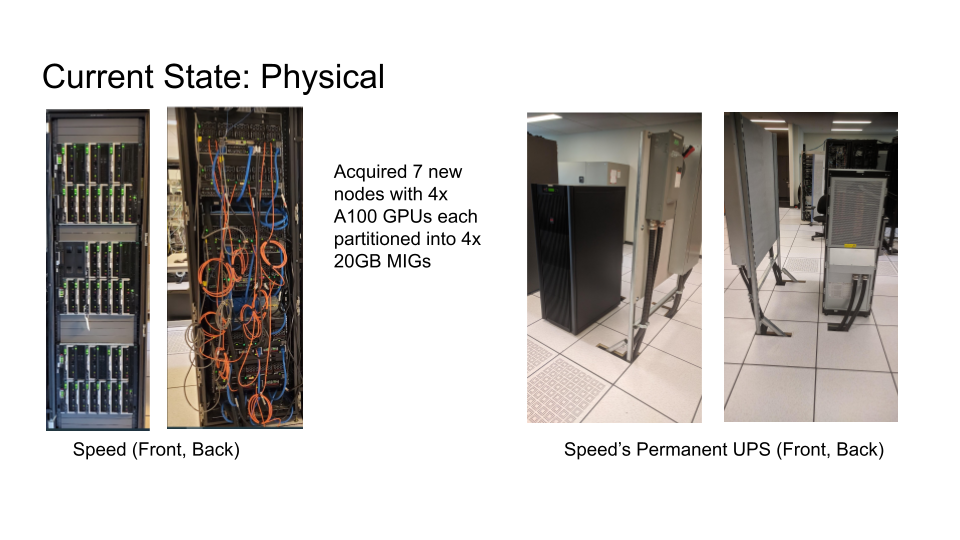
\includegraphics[width=\columnwidth]{images/speed-pics}
\caption{Speed}
\label{fig:speed-pics}
\end{figure}

\begin{figure}[htpb]
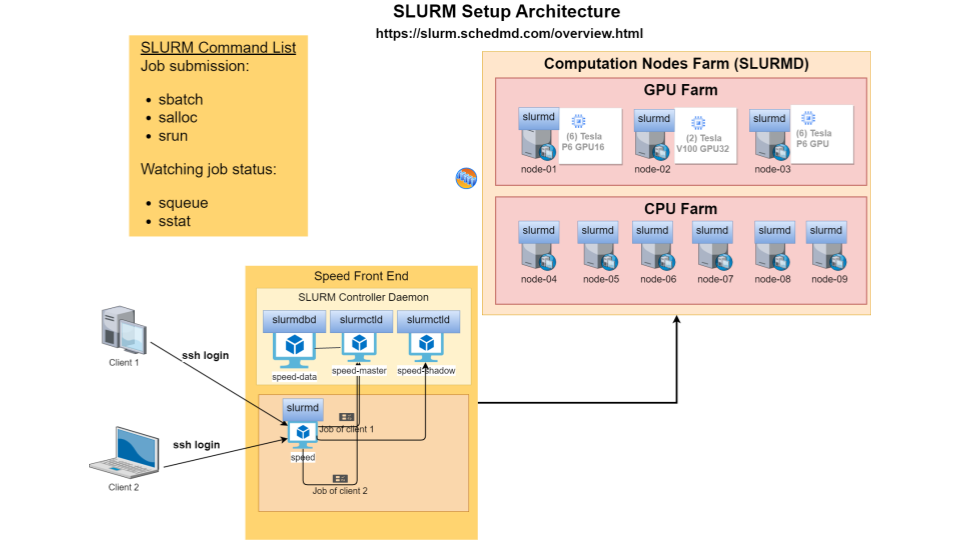
\includegraphics[width=\columnwidth]{images/slurm-arch}
\caption{Speed SLURM Architecture}
\label{fig:slurm-arch}
\end{figure}


% ------------------------------------------------------------------------------
\subsection{What Speed Is Ideal For}
\label{sect:speed-is-for}

\begin{itemize}
\item
To design and develop, test and run parallel, batch, and other algorithms, 
scripts with partial data sets. ``Speed'' has been optimised for compute jobs 
that are multi-core aware, require a large memory space, or are iteration 
intensive.
\item
Prepare them for big clusters:
	\begin{itemize}
	\item 
	Digital Research Alliance of Canada (Calcul Quebec and Compute Canada)
	\item 
	Cloud platforms
	\end{itemize}
\item
Jobs that are too demanding for a desktop. 
\item
Single-core batch jobs; multithreaded jobs typically up to 32 cores (i.e., a single machine).
\item
Multi-node multi-core jobs (MPI).
\item
Anything that can fit into a 500-GB memory space and a \textbf{scratch} space of approximately 10~TB. 
\item
CPU-based jobs. 
\item
CUDA GPU jobs (\texttt{speed-01|-03|-05}, \texttt{speed-17}, \texttt{speed-37}--\texttt{speed-43}).
\item
Non-CUDA GPU jobs using OpenCL (\texttt{speed-19} and \texttt{-01|03|05|17|25|27|37-43}).
\end{itemize}

% ------------------------------------------------------------------------------
\subsection{What Speed Is Not}
\label{sect:speed-is-not}

\begin{itemize}
\item Speed is not a web host and does not host websites.
\item Speed is not meant for Continuous Integration (CI) automation deployments for Ansible or similar tools. 
\item Does not run Kubernetes or other container orchestration software.
\item Does not run Docker. (\textbf{Note:} Speed does run Singularity and many Docker containers can be converted to Singularity containers with a single command. See \xs{sect:singularity-containers}.)
\item Speed is not for jobs executed outside of the scheduler. (Jobs running outside of the scheduler will be killed and all data lost.)
\end{itemize}

% ------------------------------------------------------------------------------
\subsection{Available Software}

We have a great number of open-source software available and installed
on ``Speed''~--~various Python, CUDA versions, {\cpp}/{\java} compilers, OpenGL,
OpenFOAM, OpenCV, TensorFlow, OpenMPI, OpenISS, {\marf}~\cite{marf}, etc.
There are also a number of commercial packages, subject to licensing
contributions, available, such as MATLAB~\cite{matlab,scholarpedia-matlab}, Abaqus~\cite{abaqus}, 
Ansys, Fluent~\cite{fluent}, etc. 

To see the packages available, run \texttt{ls -al /encs/pkg/} on \texttt{speed.encs}.
%
In particular, there are over 2200 programs available in
\texttt{/encs/bin} and \texttt{/encs/pkg} under Scientific Linux 7 (EL7).
We are building an equivalent array of programs for the EL9 SPEED2 nodes.

\begin{itemize}
	\item 
Popular concrete examples:
\begin{itemize}
	\item 
MATLAB (R2016b, R2018a, R2018b, ...)
	\item 
Fluent (19.2, ...)
	\item 
Singularity containers (see \xs{sect:singularity-containers}) can run other 
operating systems and Linux distributions, like Ubuntu's, as well as 
converted Docker containers.
\end{itemize}
	\item 
We do our best to accommodate custom software requests.
Python environments can use user-custom installs 
from within the scratch directory.
	\item 
A number of specific environments are available and 
can be loaded using the \tool{module} command:
\begin{itemize}
	\item 
Python (2.3.x - 3.11.x)
	\item 
Gurobi (7.0.1, 7.5.0, 8.0.0, 8.1.0)
	\item 
Ansys (16, 17, 18, 19)
	\item 
OpenFOAM (2.3.1, 3.0.1, 5.0, 6.0)
	\item 
Cplex 12.6.x to 12.8.x
	\item 
OpenMPI 1.6.x, 1.8.x, 3.1.3
\end{itemize}
\end{itemize}

% ------------------------------------------------------------------------------
\subsection{Requesting Access}
\label{sect:access}

After reviewing the ``What Speed is'' (\xs{sect:speed-is-for}) and
``What Speed is Not'' (\xs{sect:speed-is-not}), request access to the ``Speed'' 
cluster by emailing: \texttt{rt-ex-hpc AT encs.concordia.ca}.
%
CGS ENCS faculty and staff may request access directly.
Students must include the following in their message:

\begin{itemize} 
	\item GCS ENCS username
	\item Name and email (CC) of the supervisor or instructor
	\item Written request from the supervisor or instructor for the ENCS username to be granted access to ``Speed''
\end{itemize}

Non-GCS faculty / students need to get a ``sponsor'' within GCS, such that
your guest GCS ENCS account is created first. A sponsor can be any GCS Faculty member
you collaborate with. Failing that, request the approval from our Dean's Office;
via our Associate Deans Drs.\ Eddie Hoi Ng or Emad Shihab.
%
External entities to Concordia who collaborate with CGS Concordia researchers,
should also go through the Dean's office for approvals.
%
Non-GCS students taking a GCS course do have their GCS ENCS account created automatically,
but still need the course instructor's approval to use the service.

% ------------------------------------------------------------------------------
\section{Job Management}
\label{sect:job-management}

In these instructions, anything bracketed like so, \verb+<>+, indicates a
label/value to be replaced (the entire bracketed term needs replacement).
%
We use SLURM as the Workload Manager.
It supports primarily two types of jobs: batch and interactive.
Batch jobs are used to run unattended tasks.

TL;DR:
Job instructions in a script start with \verb+#SBATCH+ prefix, for example:
\begin{verbatim}
#SBATCH --account=speed1 --mem=100M -t 600 -J job-name
#SBATCH --gpus=2 --mail-type=ALL -t 600 --mail-user=YOUR_USERNAME
\end{verbatim}
%
We use \tool{srun} for every complex compute step inside the script.
Use interactive jobs to set up virtual environments, compilation, and debugging.
\tool{salloc} is preferred; allows multiple steps.
\tool{srun} can start interactive jobs as well (see \xs{sect:interactive-jobs}).
Required and common job parameters: job-name (J), mail-type, mem, ntasks (n),
cpus-per-task, account, -p (partition).


% ------------------------------------------------------------------------------
\subsection{Getting Started}

Before getting started, please review the ``What Speed is'' (\xs{sect:speed-is-for})
and ``What Speed is Not'' (\xs{sect:speed-is-not}).
Once your GCS ENCS account has been granted access to ``Speed'',
use your GCS ENCS account credentials to create an SSH connection to 
\texttt{speed} (an alias for \texttt{speed-submit.encs.concordia.ca}). 
%
All users are expected to have a basic understanding of
Linux and its commonly used commands (see \xa{sect:faqs-linux} for resources).

% ------------------------------------------------------------------------------
\subsubsection{SSH Connections}
\label{sect:ssh}

Requirements to create connections to Speed:
\begin{enumerate}
	\item
An active \textbf{GCS ENCS user account}, which has permission to connect to Speed
(see \xs{sect:access}).
	\item
If you are off campus, an active connection to Concordia's VPN.
Accessing Concordia's VPN requires a Concordia \textbf{netname}. 
	\item
Windows systems require a terminal emulator such as PuTTY, Cygwin, or MobaXterm.
	\item
macOS systems do have a Terminal app for this or \tool{xterm} that comes with XQuarz.
\end{enumerate}

Open up a terminal window and type in the following SSH command being sure to replace
\verb!<ENCSusername>! with your ENCS account's username.

\begin{verbatim}
ssh <ENCSusername>@speed.encs.concordia.ca
\end{verbatim}

\noindent
Read the AITS FAQ:
\href
{https://www.concordia.ca/ginacody/aits/support/faq/ssh-to-gcs.html}
{How do I securely connect to a GCS server?}


% ------------------------------------------------------------------------------
% TMP scheduler-specific section
% ------------------------------------------------------------------------------
\subsubsection{Environment Set Up}
\label{sect:envsetup}

After creating an SSH connection to ``Speed'', you will need to
make sure the \tool{srun}, \tool{sbatch}, and \tool{salloc}
commands are available to you. 
Type the command name at the linux prompt and press enter.
If the command is not available, e.g.,  (``command not found'') is returned,
you need to make sure your \api{\$PATH} has \texttt{/local/bin} in it.
To view your \api{\$PATH} type \texttt{echo \$PATH} at the linux prompt.
%
%source 
%the ``Altair Grid Engine (AGE)'' scheduler's settings file. 
%Sourcing the settings file will set the environment variables required to 
%execute scheduler commands.
%
%Based on the UNIX shell type, choose one of the following commands to source
%the settings file. 
%
%csh/\tool{tcsh}:
%\begin{verbatim}
%source /local/pkg/uge-8.6.3/root/default/common/settings.csh 
%\end{verbatim}
%
%Bourne shell/\tool{bash}:
%\begin{verbatim}
%. /local/pkg/uge-8.6.3/root/default/common/settings.sh 
%\end{verbatim}
%
%In order to set up the default ENCS bash shell, executing the following command 
%is also required:
%\begin{verbatim}
%printenv ORGANIZATION | grep -qw ENCS || . /encs/Share/bash/profile 
%\end{verbatim}
%
%To verify that you have access to the scheduler commands execute 
%\texttt{qstat -f -u "*"}. If an error is returned, attempt sourcing 
%the settings file again.

The next step is to copy a job template to your home directory and to set up your
cluster-specific storage. Execute the following command from within your
home directory. (To move to your home directory, type \texttt{cd} at the Linux
prompt and press \texttt{Enter}.) 

\begin{verbatim}
cp /home/n/nul-uge/template.sh . && mkdir /speed-scratch/$USER
\end{verbatim}

%\textbf{Tip:} Add the source command to your shell-startup script. 

\textbf{Tip:} the default shell for GCS ENCS users is \tool{tcsh}.
If you would like to use \tool{bash}, please contact 
\texttt{rt-ex-hpc AT encs.concordia.ca}.

%For \textbf{new GCS ENCS Users}, and/or those who don't have a shell-startup script, 
%based on your shell type use one of the following commands to copy a start up script 
%from \texttt{nul-uge}'s home directory to your home directory. (To move to your home
%directory, type \tool{cd} at the Linux prompt and press \texttt{Enter}.)

%csh/\tool{tcsh}:
%\begin{verbatim}
%cp /home/n/nul-uge/.tcshrc . 
%\end{verbatim}

%Bourne shell/\tool{bash}:
%\begin{verbatim}
%cp /home/n/nul-uge/.bashrc . 
%\end{verbatim}

%Users who already have a shell-startup script, can use a text editor, such as
%\tool{vim} or \tool{emacs}, to add the source request to your existing
%shell-startup environment (i.e., to the \file{.tcshrc} file in your home directory). 

%csh/\tool{tcsh}:
%Sample \file{.tcshrc} file:
%\begin{verbatim}
%# Speed environment set up 
%if ($HOSTNAME == speed-submit.encs.concordia.ca) then
   %source /local/pkg/uge-8.6.3/root/default/common/settings.csh
%endif
%\end{verbatim}
%
%Bourne shell/\tool{bash}:
%Sample \file{.bashrc} file:
%\begin{verbatim}
%# Speed environment set up 
%if [ $HOSTNAME = "speed-submit.encs.concordia.ca" ]; then
    %. /local/pkg/uge-8.6.3/root/default/common/settings.sh
    %printenv ORGANIZATION | grep -qw ENCS || . /encs/Share/bash/profile
%fi
%\end{verbatim}

%\noindent
%\textbf{NOTE:} If you have used UGE commands in the past you probably still have these
%lines there; \textbf{they should now be removed}, as they have no use in SLURM:

%csh/\tool{tcsh}:
%Sample \file{.tcshrc} file:
%\begin{verbatim}
%# Speed environment set up 
%if ($HOSTNAME == speed-submit.encs.concordia.ca) then
%   source /local/pkg/uge-8.6.3/root/default/common/settings.csh
%endif
%\end{verbatim}

%Bourne shell/\tool{bash}:
%Sample \file{.bashrc} file:
%\begin{verbatim}
%# Speed environment set up 
%if [ $HOSTNAME = "speed-submit.encs.concordia.ca" ]; then
%    . /local/pkg/uge-8.6.3/root/default/common/settings.sh
%    printenv ORGANIZATION | grep -qw ENCS || . /encs/Share/bash/profile
%fi
%\end{verbatim}

%Note that you will need to either log out and back in, or execute a new shell, 
%for the environment changes in the updated \file{.tcshrc} or \file{.bashrc} file to be applied 
%(\textbf{important}).


% ------------------------------------------------------------------------------
\subsection{Job Submission Basics}

Preparing your job for submission is fairly straightforward.
Start by basing your job script on one of the examples available in the \texttt{src/}
directory of our GitHub's (\url{https://github.com/NAG-DevOps/speed-hpc}).
%
Job scripts are broken into four main sections: 

\begin{itemize}
	\item Directives
	\item Module Loads
	\item User Scripting
\end{itemize}

You can clone the tip of our repository to get the examples to start
with or download them individually via a browser or command line:

\small
\begin{verbatim}
git clone --depth=1 https://github.com/NAG-DevOps/speed-hpc.git
cd speed-hpc/src
\end{verbatim}
\normalsize

\noindent
Then to quickly run some sample jobs, you can:
\small
\begin{verbatim}
sbatch -p ps -t 10 bash.sh
sbatch -p ps -t 10 env.sh
sbatch -p ps -t 10 manual.sh
sbatch -p pg -t 10 lambdal-singularity.sh
\end{verbatim}
\normalsize


% ------------------------------------------------------------------------------
% TMP scheduler-specific section
% ------------------------------------------------------------------------------
\subsubsection{Directives}
\label{sect:directives}

Directives are comments included at the beginning of a job script that set the shell 
and the options for the job scheduler. 
%
The shebang directive is always the first line of a script. In your job script, 
this directive sets which shell your script's commands will run in. On ``Speed'', 
we recommend that your script use a shell from the \texttt{/encs/bin} directory. 

To use the \texttt{tcsh} shell, start your script with \verb|#!/encs/bin/tcsh|.
%
For \texttt{bash}, start with \verb|#!/encs/bin/bash|.
%
Directives that start with \verb|#SBATCH|, set the options for the cluster's 
Slurm job scheduler. The script template, \texttt{template.sh}, 
provides the essentials:

%\begin{verbatim}
%#$ -N <jobname>
%#$ -cwd
%#$ -m bea
%#$ -pe smp <corecount>
%#$ -l h_vmem=<memory>G
%\end{verbatim}
\begin{verbatim}
#SBATCH --job-name=<jobname>        ## or -J. Give the job a name 
#SBATCH --mail-type=<type>          ## Set type of email notifications
#SBATCH --chdir=<directory>         ## or -D, Set working directory where output files will go 
#SBATCH --nodes=1                   ## or -N, Node count required for the job
#SBATCH --ntasks=1                  ## or -n, Number of tasks to be launched
#SBATCH --cpus-per-task=<corecount> ## or -c, Core count requested, e.g. 8 cores
#SBATCH --mem=<memory>              ## Assign memory for this job, e.g., 32G memory per node 
\end{verbatim}

Replace the following to adjust the job script for your project(s)
\begin{enumerate}
  \item \verb+<jobname>+ with a job name for the job
  \item \verb+<directory>+ with the fullpath to your job's working directory, e.g., where your code,
source files and where the standard output files will be written to. By default, \verb+--chdir+
sets the current directory as the job's working directory 
  \item \verb+<type>+ with the type of e-mail notifications you wish to receive. Valid options are: NONE, BEGIN, END, FAIL, REQUEUE, ALL 
  \item \verb+<corecount>+ with the degree of multithreaded parallelism (i.e., cores) allocated to your job. Up to 32 by default.
  \item \verb+<memory>+ with the amount of memory, in GB, that you want to be allocated per node. Up to 500 depending on the node. 
  NOTE: All jobs MUST set a value for the \verb|--mem| option.
\end{enumerate}

Example with short option equivalents:

\begin{verbatim}
#SBATCH -J tmpdir                   ## Job's name set to 'tmpdir'
#SBATCH --mail-type=ALL             ## Receive all email type notifications
#SBATCH -D ./                       ## Use current directory as working directory
#SBATCH -N 1                        ## Node count required for the job
#SBATCH -n 1                        ## Number of tasks to be launched
#SBATCH -c 8                        ## Request 8 cores
#SBATCH --mem=32G                   ## Allocate 32G memory per node 
\end{verbatim}

%
If you are unsure about memory footprints, err on assigning a generous
memory space to your job, so that it does not get prematurely terminated.
%(the value given to \api{h\_vmem} is a hard memory ceiling).
You can refine
%\api{h\_vmem}
\option{--mem}
values for future jobs by monitoring the size of a job's active
memory space on \texttt{speed-submit} with:

%\begin{verbatim}
%qstat -j <jobID> | grep maxvmem
%\end{verbatim}

\begin{verbatim}
sacct -j <jobID>
sstat -j <jobID>
\end{verbatim}

\noindent
This can be customized to show specific columns:

\begin{verbatim}
sacct -o jobid,maxvmsize,ntasks%7,tresusageouttot%25 -j <jobID>
sstat -o jobid,maxvmsize,ntasks%7,tresusageouttot%25 -j <jobID>
\end{verbatim}

Memory-footprint values are also provided for completed jobs in the final
e-mail notification as ``maxvmsize''.
%
\emph{Jobs that request a low-memory footprint are more likely to load on a busy
cluster.}

Other essential options are \option{--time}, or \verb|-t|, and \option{--account}, or \verb|-A|.
%
\begin{itemize}
\item
\option{--time=<time>} -- is the estimate of wall clock time required for your job to run. 
As preiviously mentioned, the maximum is 7 days for batch and 24 hours for interactive jobs. 
Jobs with a smaller \texttt{time} value will have a higher priority and may result in your job being scheduled sooner. 

\item
\option{--account=<name>} -- specifies which Account, aka project or association, 
that the Speed resources your job uses should be attributed to. When moving from 
GE to SLURM users most users were assigned to Speed's two default accounts 
\texttt{speed1} and \texttt{speed2}. However, users that belong to a particular research
group or project are will have a default Account like the following
\texttt{aits},
\texttt{vidpro},
\texttt{gipsy},
\texttt{ai2},
\texttt{mpackir},
\texttt{cmos}, among others.

\end{itemize}

% ------------------------------------------------------------------------------
\subsubsection{Module Loads}
\label{sect:modules}

As your job will run on a compute or GPU ``Speed'' node, and not the submit node,
any software that is needed must be loaded by the job script. Software is loaded
within the script just as it would be from the command line.

To see a list of which modules are available, execute the following from the 
command line on \texttt{speed-submit}.

\begin{verbatim}
module avail
\end{verbatim}

To list for a particular program (\tool{matlab}, for example):

\begin{verbatim}
module -t avail matlab
\end{verbatim}

Which, of course, can be shortened to match all that start with a
particular letter:

\begin{verbatim}
module -t avail m
\end{verbatim}

Insert the following in your script to load the \tool{matlab/R2020a}) module:

\begin{verbatim}
module load matlab/R2020a/default
\end{verbatim}

Use, \option{unload}, in place of, \option{load}, to remove a module from active use.

To list loaded modules:

\begin{verbatim}
module list
\end{verbatim}

To purge all software in your working environment:

\begin{verbatim}
module purge
\end{verbatim}

Typically, only the \texttt{module load} command will be used in your script.

% ------------------------------------------------------------------------------
% TMP scheduler-specific section
% ------------------------------------------------------------------------------
\subsubsection{User Scripting}
\label{sect:scripting}

The last part the job script is the scripting that will be executed by the job. 
This part of the job script includes all commands required to set up and 
execute the task your script has been written to do. Any Linux command can be used 
at this step. This section can be a simple call to an executable or a complex 
loop which iterates through a series of commands.

Any compute heavy step is preferably should be prefixed by \tool{srun}
as the best practice.

Every software program has a unique execution framework. It is the responsibility 
of the script's author (e.g., you) to know what is required for the software used 
in your script by reviewing the software's documentation. Regardless of which software
your script calls, your script should be written so that the software knows the 
location of the input and output files as well as the degree of parallelism.
%
% GE:
%Note that the cluster-specific environment variable, \api{NSLOTS}, resolves 
%to the value provided to the scheduler in the \option{-pe smp} option. 

Jobs which touch data-input and data-output files more than once, should make use 
of \api{TMPDIR}, a scheduler-provided working space almost 1~TB in size.
\api{TMPDIR} is created when a job starts, and exists on the local disk of the
compute node executing your job. Using \api{TMPDIR} results in faster I/O operations 
than those to and from shared storage (which is provided over NFS). 

An sample job script using \api{TMPDIR} is available at \texttt{/home/n/nul-uge/templateTMPDIR.sh}: 
the job is instructed to change to \api{\$TMPDIR}, to make the new directory \texttt{input}, to copy data from
%\texttt{\$SGE\_O\_WORKDIR/references/} to \texttt{input/} (\texttt{\$SGE\_O\_WORKDIR} represents the
\texttt{\$SLURM\_SUBMIT\_DIR/references/} to \texttt{input/} (\texttt{\$SLURM\_SUBMIT\_DIR} represents the
current working directory), to make the new directory \texttt{results}, to
execute the program (which takes input from \texttt{\$TMPDIR/input/} and writes
output to \texttt{\$TMPDIR/results/}), and finally to copy the total end results
to an existing directory, \texttt{processed}, that is located in the current
working directory.
% TODO: verify:
TMPDIR only exists for the duration of the job, though,
so it is very important to copy relevant results from it at job's end.

% ------------------------------------------------------------------------------
\subsection{Sample Job Script}

Now, let's look at a basic job script, \file{tcsh.sh} in \xf{fig:tcsh.sh}
(you can copy it from our GitHub page or from \texttt{/home/n/nul-uge}).

\begin{figure}[htpb]
	\lstinputlisting[language=csh,frame=single,basicstyle=\ttfamily]{tcsh.sh}
	\caption{Source code for \file{tcsh.sh}}
	\label{fig:tcsh.sh}
\end{figure}

The first line is the shell declaration (also know as a shebang) and sets the shell to \emph{tcsh}.
%The lines that begin with \texttt{\#\$} are directives for the scheduler.
The lines that begin with \texttt{\#SBATCH} are directives for the scheduler.

\begin{itemize}
	%\item \texttt{-N} sets \emph{qsub-test} as the jobname
	\item \texttt{-J} (or \option{--job-name}) sets \emph{tcsh-test} as the job name
	%\item \texttt{-cwd} tells the scheduler to execute the job from the current working directory
	\item \texttt{--chdir} tells the scheduler to execute the job from the current working directory
	%\item \texttt{-l h\_vmem=1GB} requests and assigns 1GB of memory to the job. CPU jobs \emph{require} the \texttt{-l h\_vmem} option to be set.
	\item \texttt{--mem=1GB} requests and assigns 1GB of memory to the job. 
	Jobs \emph{require} the \texttt{--mem} option to be set either in the script
	or on the command line; \textbf{if it's missing job submission will be rejected.}
\end{itemize}

The script then:

\begin{itemize}
	\item Sleeps on a node for 30 seconds
	\item Uses the \tool{module} command to load the \texttt{gurobi/8.1.0} environment
	\item Prints the list of loaded modules into a file
\end{itemize}

%The scheduler command, \tool{qsub}, is used to submit (non-interactive) jobs. 
The scheduler command, \tool{sbatch}, is used to submit (non-interactive) jobs. 
%From an ssh session on speed-submit, submit this job with \texttt{qsub ./tcsh.sh}.
From an ssh session on speed-submit, submit this job with \texttt{sbatch ./tcsh.sh}.
%You will see, \texttt{"Your job X ("qsub-test") has been submitted"}.
You will see, \texttt{"Submitted batch job 2653"} where $2653$ is a job ID assigned.
%The command, \tool{qstat}, can be used 
The commands, \tool{squeue} and \tool{sinfo} can be used 
%to look at the status of the cluster: \texttt{qstat -f -u "*"}.
to look at the status of the cluster: \texttt{squeue -l}.
You will see something like this: 

%\small
%\begin{verbatim}
%queuename                      qtype resv/used/tot. load_avg arch          states
%---------------------------------------------------------------------------------
%a.q@speed-01.encs.concordia.ca BIP   0/0/32         0.01     lx-amd64
%---------------------------------------------------------------------------------
%a.q@speed-03.encs.concordia.ca BIP   0/0/32         0.01     lx-amd64
%---------------------------------------------------------------------------------
%a.q@speed-25.encs.concordia.ca BIP   0/0/32         0.01     lx-amd64
%---------------------------------------------------------------------------------
%a.q@speed-27.encs.concordia.ca BIP   0/0/32         0.01     lx-amd64
%---------------------------------------------------------------------------------
%g.q@speed-05.encs.concordia.ca BIP   0/0/32         0.02     lx-amd64
     %144   100.00000 qsub-test nul-uge     r     12/03/2018 16:39:30    1 
     %62624 0.09843 case_talle x_yzabc      r     11/09/2021 16:50:09    32
%---------------------------------------------------------------------------------
%g.q@speed-17.encs.concordia.ca BIP   0/0/32         0.01     lx-amd64
%---------------------------------------------------------------------------------
%s.q@speed-07.encs.concordia.ca BIP   0/0/32         0.04     lx-amd64
%---------------------------------------------------------------------------------
%s.q@speed-08.encs.concordia.ca BIP   0/0/32         0.01     lx-amd64
%---------------------------------------------------------------------------------
%s.q@speed-09.encs.concordia.ca BIP   0/0/32         0.01     lx-amd64
%---------------------------------------------------------------------------------
%s.q@speed-10.encs.concordia.ca BIP   0/32/32        32.72    lx-amd64
     %62624 0.09843 case_talle x_yzabc      r     11/09/2021 16:50:09    32
%---------------------------------------------------------------------------------
%s.q@speed-11.encs.concordia.ca BIP   0/32/32        32.08    lx-amd64
     %62679 0.14212 CWLR_DF    a_bcdef      r     11/10/2021 17:25:19    32
%---------------------------------------------------------------------------------
%s.q@speed-12.encs.concordia.ca BIP   0/32/32        32.10    lx-amd64
     %62749 0.09000 CLOUDY     z_abc        r     11/11/2021 21:58:12    32
%---------------------------------------------------------------------------------
%s.q@speed-15.encs.concordia.ca BIP   0/4/32         0.03     lx-amd64
     %62753 82.47478 matlabLDPa b_bpxez      r     11/12/2021 08:49:52     4
%---------------------------------------------------------------------------------
%s.q@speed-16.encs.concordia.ca BIP   0/32/32        32.31    lx-amd64
     %62751 0.09000 CLOUDY     z_abc        r     11/12/2021 06:03:54    32
%---------------------------------------------------------------------------------
%s.q@speed-19.encs.concordia.ca BIP   0/32/32        32.22    lx-amd64
%---------------------------------------------------------------------------------
%...
%---------------------------------------------------------------------------------
%s.q@speed-35.encs.concordia.ca BIP   0/32/32        2.78     lx-amd64
     %62754 7.22952 qlogin-tes a_tiyuu      r     11/12/2021 10:31:06    32
%---------------------------------------------------------------------------------
%s.q@speed-36.encs.concordia.ca BIP   0/0/32         0.03     lx-amd64
%etc.
\small
\begin{verbatim}
[serguei@speed-submit src] % squeue -l
Thu Oct 19 11:38:54 2023
JOBID PARTITION     NAME     USER    STATE       TIME TIME_LIMI  NODES NODELIST(REASON)
 2641        ps interact   b_user  RUNNING   19:16:09 1-00:00:00      1 speed-07
 2652        ps interact   a_user  RUNNING      41:40 1-00:00:00      1 speed-07
 2654        ps tcsh-tes  serguei  RUNNING       0:01 7-00:00:00      1 speed-07
[serguei@speed-submit src] % sinfo
PARTITION AVAIL  TIMELIMIT  NODES  STATE NODELIST
ps*          up 7-00:00:00     14  drain speed-[08-10,12,15-16,20-22,30-32,35-36]
ps*          up 7-00:00:00      1    mix speed-07
ps*          up 7-00:00:00      7   idle speed-[11,19,23-24,29,33-34]
pg           up 1-00:00:00      1  drain speed-17
pg           up 1-00:00:00      3   idle speed-[05,25,27]
pt           up 7-00:00:00      7   idle speed-[37-43]
pa           up 7-00:00:00      4   idle speed-[01,03,25,27]
\end{verbatim}
\normalsize

Remember that you only have 30 seconds before the job is essentially over, so 
if you do not see a similar output, either adjust the sleep time in the 
%script, or execute the \tool{qstat} statement more quickly. The \tool{qstat} 
script, or execute the \tool{sbatch} statement more quickly. The \tool{squeue} 
output listed above shows you that your job is 
running on node \texttt{speed-07}, that it has a job number of 2654,
its time limit of 7 days, etc.
% TODO
%, that it 
%was started at 16:39:30 on 12/03/2018, and that it is a single-core job (the 
%default). 

Once the job finishes, there will be a new file in the directory that the job 
%was started from, with the syntax of, \texttt{"job name".o"job number"}, so 
was started from, with the syntax of, \texttt{slurm-"job id".out}, so 
%in this example the file is, qsub \file{test.o144}. This file represents the 
in this example the file is, \file{slurm-2654.out}. This file represents the 
standard output (and error, if there is any) of the job in question. If you 
look at the contents of your newly created file, you will see that it 
contains the output of the, \texttt{module list} command. 
Important information is often written to this file.
%
%Congratulations on your first job! 

% ------------------------------------------------------------------------------
\subsection{Common Job Management Commands Summary}
\label{sect:job-management-commands}

Here are useful job-management commands: 

\begin{itemize}
%\item
%\texttt{qsub ./<myscript>.sh}: once that your job script is ready,
%on \texttt{speed-submit} you can submit it using this
\item
\texttt{sbatch -A <ACCOUNT> --t <MINUTES> --mem=20G -p <PARTITION> ./<myscript>.sh}: once that your job script is ready,
on \texttt{speed-submit} you can submit it using this

\item
%\texttt{qstat -f -u <ENCSusername>}: you can check the status of your job(s)
\texttt{squeue -u <ENCSusername>}: you can check the status of your job(s)

\item
%\texttt{qstat -f -u "*"}: display cluster status for all users. 
\texttt{squeue}: display cluster status for all users. 
\option{-A} shows per account (e.g., \texttt{vidpro}, \texttt{gipsy},
\texttt{speed1}, \texttt{ai2}, \texttt{aits}, etc.),
\option{-p} per partition (\texttt{ps}, \texttt{pg}, \texttt{pt}, \texttt{pa}),
and others. \texttt{man squeue} for details.

\item
%\texttt{qstat -j [job-ID]}: display job information for [job-ID] (said job may be actually running, or waiting in the queue). 
\texttt{squeue --job [job-ID]}: display job information for [job-ID] (said job may be actually running, or waiting in the queue). 

\item
\texttt{squeue -las}: displays individual job steps (for debugging
easier to see which step failed if you used \tool{srun}).

\item
\verb+watch -n 1 "sinfo -Nel -pps,pt,pg,pa && squeue -la"+: view \tool{sinfo} information and watch the queue for your job(s).

%\item
%\texttt{qdel [job-ID]}: delete job [job-ID]. 
\item
\texttt{scancel [job-ID]}: cancel job [job-ID]. 

%\item
%\texttt{qhold [job-ID]}: hold queued job, [job-ID], from running. 
\item
\texttt{scontrol hold [job-ID]}: hold queued job, [job-ID], from running. 

%\item
%\texttt{qrls [job-ID]}: release held job [job-ID]. 
\item
\texttt{scontrol release [job-ID]}: release held job [job-ID]. 

\item
%\texttt{qacct -j [job-ID]}: get job stats. for completed job [job-ID]. \api{maxvmem} is one of the more useful stats. 
\texttt{sacct -j [job-ID]}: get job stats.
%for completed job [job-ID].
\api{maxvmem} is one of the more useful stats that you can elect to display
as a format option.

\small
\begin{verbatim}
% sacct -j 2654
JobID           JobName  Partition    Account  AllocCPUS      State ExitCode
------------ ---------- ---------- ---------- ---------- ---------- --------
2654          tcsh-test         ps     speed1          1  COMPLETED      0:0
2654.batch        batch                speed1          1  COMPLETED      0:0
2654.extern      extern                speed1          1  COMPLETED      0:0
% sacct -j 2654 -o jobid,user,account,MaxVMSize,Reason%10,TRESUsageOutMax%30
JobID             User    Account  MaxVMSize     Reason        TRESUsageOutMax
------------ --------- ---------- ---------- ---------- ----------------------
2654           serguei     speed1                  None
2654.batch                 speed1    296840K             energy=0,fs/disk=1975
2654.extern                speed1    296312K              energy=0,fs/disk=343
\end{verbatim}
\normalsize

See \texttt{man sacct} or \texttt{sacct -e} for details of the
available formatting options. You can define your preferred
default format in the \api{SACCT\_FORMAT} environment variable
in your \texttt{.cshrc} or \texttt{.bashrc} files.

\end{itemize}


% ------------------------------------------------------------------------------
%\subsection{Advanced \tool{qsub} Options}
\subsection{Advanced \tool{sbatch} Options}
\label{sect:submit-options}
\label{sect:qsub-options}

In addition to the basic \tool{sbatch} options presented earlier, there are a 
few additional options that are generally useful:

\begin{itemize}
\item
%\texttt{-m bea}: requests that the scheduler e-mail you when a job (b)egins;
%(e)nds; (a)borts. Mail is sent to the default address of,
%\texttt{"username@encs.concordia.ca"}, unless a different address is supplied (see, 
%\texttt{-M}). The report sent when a job ends includes job 
%runtime, as well as the maximum memory value hit (\api{maxvmem}). 
\texttt{--mail-type=TYPE}: requests that the scheduler e-mail you when a job changes
state. Where \texttt{TYPE} is \texttt{ALL}, \texttt{BEGIN}, \texttt{END}, or \texttt{FAIL}.
% TODO: verify
Mail is sent to the default address of, \\
\texttt{"<ENCSusername>@encs.concordia.ca"}, which you can consult
via \texttt{webmail.encs} via the VPN, on login.encs via \tool{alpine}
or setup forwarding to @concordia.ca address or offsite,
unless a different address is supplied (see, \texttt{--mail-user}).
% TODO: double-check
The report sent when a job ends includes job 
runtime, as well as the maximum memory value hit (\api{maxvmem}). 

\item
%\texttt{-M email@domain.com}: requests that the scheduler use this e-mail 
%notification address, rather than the default (see, \texttt{-m}). 
\texttt{--mail-user email@domain.com}: requests that the scheduler use this e-mail 
notification address, rather than the default (see, \texttt{--mail-type}). 

\item
%\texttt{-v variable[=value]}: exports an environment variable that can be used by the script.
\texttt{--export=[ALL | NONE | variables]}: exports environment variable(s) that can be used by the script.

\item
%\texttt{-l h\_rt=[hour]:[min]:[sec]}: sets a job runtime of HH:MM:SS. Note 
%that if you give a single number, that represents \emph{seconds}, not hours. 
\texttt{-t [min]} or \texttt{DAYS-HH:MM:SS}: sets a job runtime of min or HH:MM:SS. Note 
that if you give a single number, that represents \emph{minutes}, not hours. 

\item
%\texttt{-hold\_jid [job-ID]}: run this job only when job [job-ID] finishes. Held jobs appear in the queue. 
\texttt{--depend=[state:job-ID]}: run this job only when job [job-ID] finishes. Held jobs appear in the queue. 

\end{itemize}

The many \tool{sbatch} options available are read with, \texttt{man sbatch}. Also 
note that \tool{sbatch} options can be specified during the job-submission 
command, and these \emph{override} existing script options (if present). The 
syntax is, \texttt{sbatch [options] PATHTOSCRIPT}, but unlike in the script, 
the options are specified without the leading \verb+#SBATCH+
(e.g., \texttt{sbatch -J sub-test --chdir=./ --mem=1G ./tcsh.sh}).


% ------------------------------------------------------------------------------
\subsection{Array Jobs}
\label{sect:array-jobs}

Array jobs are those that start a batch job or a parallel job multiple times. 
Each iteration of the job array is called a task and receives a unique job ID.
Only supported for batch jobs; submit time $< 1$ second, compared to repeatedly
submitting the same regular job over and over even from a script.

%To submit an array job, use the \texttt{\-t} option of the \texttt{qsub} 
%command as follows:
To submit an array job, use the \option{--array} option of the \texttt{sbatch} 
command as follows:

%\begin{verbatim}
%qsub -t n[-m[:s]] <batch_script>
%\end{verbatim}
\begin{verbatim}
sbatch --array=n-m[:s]] <batch_script>
\end{verbatim}

\textbf{-t Option Syntax:}
\begin{itemize}
\item
\texttt{n}: indicates the start-id.
\item
\texttt{m}: indicates the max-id.
\item
\texttt{s}: indicates the step size.
\end{itemize}

\textbf{Examples:}
\begin{itemize}
\item
\verb+sbatch --array=1-50000 -N1 -i my_in_%a -o my_out_%a array.sh+: submits a job with 50000 elements,
\%a maps to the task-id between 1 and 50K. 
\item
%\texttt{qsub -t 10 array.sh}: submits a job with 1 task where the task-id is 10. 
\texttt{sbatch --array=10 array.sh}: submits a job with 1 task where the task-id is 10. 
\item
%\texttt{qsub -t 1-10 array.sh}: submits a job with 10 tasks numbered consecutively from 1 to 10.
\texttt{sbatch --array=1-10 array.sh}: submits a job with 10 tasks numbered consecutively from 1 to 10.
\item
%\texttt{qsub -t 3-15:3 array.sh}: submits a jobs with 5 tasks numbered consecutively with step size 3
\texttt{sbatch --array=3-15:3 array.sh}: submits a jobs with 5 tasks numbered consecutively with step size 3
(task-ids 3,6,9,12,15).
\end{itemize}

\textbf{Output files for Array Jobs:}

The default and output and error-files are
%\option{job\_name.[o|e]job\_id} and\\
%\option{job\_name.[o|e]job\_id.task\_id}.
\texttt{slurm-job\_id\_task\_id.out}.
%
This means that Speed creates an output and an error-file for each task 
generated by the array-job as well as one for the super-ordinate array-job. 
To alter this behavior use the \option{-o} and \option{-e} option of
%\tool{qsub}. 
\tool{sbatch}. 

For more details about Array Job options, please review the manual pages for 
%\option{qsub} by executing the following at the command line on speed-submit 
%\tool{man qsub}.
\tool{sbatch} by executing the following at the command line on speed-submit 
\texttt{man sbatch}.
 
% ------------------------------------------------------------------------------
\subsection{Requesting Multiple Cores (i.e., Multithreading Jobs)}

For jobs that can take advantage of multiple machine cores, up to 32 cores
(per job) can be requested in your script with: 

%\begin{verbatim}
%#$ -pe smp [#cores] 
%\end{verbatim}
\begin{verbatim}
#SBATCH -n [#cores for processes] 
\end{verbatim}

or

\begin{verbatim}
#SBATCH -n 1
#SBATCH -c [#cores for threads of a single process]
\end{verbatim}

Both \tool{sbatch} and \tool{salloc} support \option{-n} on the command line,
and it should always be used either in the script or on the command line as the
default $n=1$.
\textbf{Do not request more cores than you think will be useful}, as larger-core
jobs are more difficult to schedule. On the flip side, though, if you 
are going to be running a program that scales out to the maximum single-machine
core count available, please (please) request 32 cores, to avoid node 
oversubscription (i.e., to avoid overloading the CPUs).

\textbf{Important} note about \option{--ntasks} or \option{--ntasks-per-node}
(\option{-n}) talks about processes (usually the ones ran with \tool{srun}).
\option{--cpus-per-task} (\option{-c}) corresponds to threads per process.
Some programs consider them equivalent, some don't. Fluent for example
uses \option{--ntasks-per-node=8} and \option{--cpus-per-task=1},
some just set \option{--cpus-per-task=8} and \option{--ntasks-per-node=1}.
If one of them is not $1$ then some applications need to be told to
use $n*c$ total cores.


Core count associated with a job appears under,
%``states'', in the, \texttt{qstat -f -u "*"}, output.
``AllocCPUS'', in the, \texttt{qacct -j}, output.

\small
\begin{verbatim}
[serguei@speed-submit src] % squeue -l
Thu Oct 19 20:32:32 2023
JOBID PARTITION     NAME     USER    STATE       TIME TIME_LIMI  NODES NODELIST(REASON)
 2652        ps interact   a_user  RUNNING   9:35:18 1-00:00:00      1 speed-07
[serguei@speed-submit src] % sacct -j 2652
JobID           JobName  Partition    Account  AllocCPUS      State ExitCode
------------ ---------- ---------- ---------- ---------- ---------- --------
2652         interacti+         ps     speed1         20    RUNNING      0:0
2652.intera+ interacti+                speed1         20    RUNNING      0:0
2652.extern      extern                speed1         20    RUNNING      0:0
2652.0       gydra_pmi+                speed1         20  COMPLETED      0:0
2652.1       gydra_pmi+                speed1         20  COMPLETED      0:0
2652.2       gydra_pmi+                speed1         20     FAILED      7:0
2652.3       gydra_pmi+                speed1         20     FAILED      7:0
2652.4       gydra_pmi+                speed1         20  COMPLETED      0:0
2652.5       gydra_pmi+                speed1         20  COMPLETED      0:0
2652.6       gydra_pmi+                speed1         20  COMPLETED      0:0
2652.7       gydra_pmi+                speed1         20  COMPLETED      0:0
\end{verbatim}
\normalsize

% ------------------------------------------------------------------------------
\subsection{Interactive Jobs}
\label{sect:interactive-jobs}

Job sessions can be interactive, instead of batch (script) based. Such 
sessions can be useful for testing, debugging, and optimising code and resource 
requirements, conda or python virtual environments setup, or any likewise
preparatory work prior to batch submission.

% ------------------------------------------------------------------------------
\subsubsection{Command Line}

To request an interactive job 
%session, use, \texttt{qlogin [options]}, similarly to a 
%\tool{qsub} command-line job (e.g., \texttt{qlogin -N qlogin-test -l h\_vmem=1G}).
session, use, \texttt{salloc [options]}, similarly to a 
\tool{sbatch} command-line job, e.g.,
%
\begin{verbatim}
salloc -J interactive-test --mem=1G -p ps -n 8
\end{verbatim}
%
%Note that the options that are available for \tool{qsub} are not necessarily
%available for \tool{qlogin}, notably, \texttt{-cwd}, and, \texttt{-v}. 
%
Inside the allocated \tool{salloc} session you can run shell
commands as usual; it is recommended to use \tool{srun} for
the heavy compute steps inside \tool{salloc}.
%
If it is a quick a short job just to compile something, e.g., on
a GPU node you can use an interactive \tool{srun} directly
(note no \tool{srun} can run within \tool{srun}), e.g., a 1 hour
allocation:

For \tool{tcsh}:
\begin{verbatim}
srun --pty -n 8 -p pg --gpus=1 --mem=1Gb -t 60 /encs/bin/tcsh
\end{verbatim}

For \tool{bash}:
\begin{verbatim}
srun --pty -n 8 -p pg --gpus=1 --mem=1Gb -t 60 /encs/bin/bash
\end{verbatim}

% ------------------------------------------------------------------------------
\subsubsection{Graphical Applications}

If you need to run an on-Speed graphical-based UI application (e.g., MALTLAB,
Abaqus CME, etc.), or an IDE (PyCharm, VSCode, Eclipse)
to develop and test your job's code interactively you need to enable
X11-forwarding from your client machine to speed then to the compute node.
To do so:

\begin{enumerate}
\item
you need to run an X server on your client machine, such as,
\begin{itemize}
\item on Windows: MobaXterm with X turned on, or Xming + PuTTY with X11 forwarding, or XOrg under Cygwin
\item on macOS: XQuarz -- use its \tool{xterm} and \texttt{ssh -X}
\item on Linux just use \texttt{ssh -X speed.encs.concordia.ca} 
\end{itemize}

See \url{https://www.concordia.ca/ginacody/aits/support/faq/xserver.html}
for details.

\item
verify your X connection was properly forwarded by printing the \api{DISPLAY} variable:

\verb+echo $DISPLAY+
If it has no output, then your X forwarding is not on and you may need to re-login to Speed.

\item
Use the \option{--x11} with \tool{salloc} or \tool{srun}:

\verb+salloc ... --x11=first ...+

\item
Once landed on a compute node, verify \api{DISPLAY} again.

\item
While running under scheduler, unset \api{XDG\_RUNTIME\_DIR}.

\item
Launch your graphical application:

\texttt{module load} the required version, then
\tool{matlab}, or \tool{abaqus cme}, etc.
\end{enumerate}

Here's an example of starting PyCharm (see \xf{fig:pycharm}), of which we made a sample local installation.
You can make a similar install under your own directory. If using VSCode, it's
currently only supported with the \tool{--no-sandbox} option.

\scriptsize
\begin{verbatim}
bash-3.2$ ssh -X speed (XQuartz xterm, PuTTY or MobaXterm have X11 forwarding too)
serguei@speed's password: 
[serguei@speed-submit ~] % echo $DISPLAY
localhost:14.0
[serguei@speed-submit ~] % srun -p ps --pty --x11=first --mem 4000 -t 0-06:00 /encs/bin/bash
bash-4.4$ echo $DISPLAY
localhost:77.0
bash-4.4$ hostname
speed-01.encs.concordia.ca
bash-4.4$ unset XDG_RUNTIME_DIR
bash-4.4$ /speed-scratch/nag-public/bin/pycharm.sh
\end{verbatim}
\normalsize

\begin{figure}[htpb]
			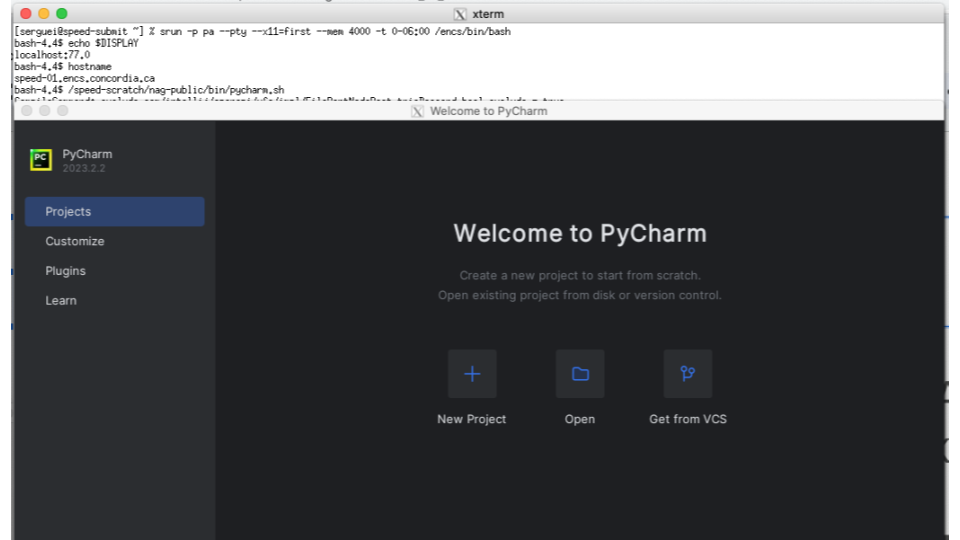
\includegraphics[width=\columnwidth]{images/pycharm}
		\caption{PyCharm Starting up on a Speed Node}
	\label{fig:pycharm}
\end{figure}

% ------------------------------------------------------------------------------
\subsubsection{Jupyter Notebooks}
\label{sect:jupyter}

This is an example of running Jupyter notebooks together with Singularity
(more on Singularity see \xs{sect:singularity-containers}).
Here we are using one of the OpenISS-derived containers (see \xs{sect:openiss-examples} as well).

\begin{enumerate}
\item
Use the \option{--x11} with \tool{salloc} or \tool{srun} as described in the above example

\item
Load Singularity module
\verb+module load singularity/3.10.4/default+

\item
Execute this Singularity command on a single line. It's best to save it in a shell script
that you could call, since it's long.
\scriptsize
\begin{verbatim}
srun singularity exec -B $PWD\:/speed-pwd,/speed-scratch/$USER\:/my-speed-scratch,/nettemp \
 --env SHELL=/bin/bash --nv /speed-scratch/nag-public/openiss-cuda-conda-jupyter.sif \
 /bin/bash -c '/opt/conda/bin/jupyter notebook --no-browser --notebook-dir=/speed-pwd \
 --ip="*" --port=8888 --allow-root'
\end{verbatim}
\normalsize

\item
Create an \tool{ssh} tunnel between your computer and the node (\texttt{speed-XX}) where Jupyter is
running (Using \texttt{speed-submit} as a ``jump server'') (Preferably: PuTTY, see \xf{fig:putty1} and \xf{fig:putty2})
\begin{verbatim}
ssh -L 8888:localhost:8888 speed-XX
\end{verbatim}
Don't close the tunnel.

\item
Open a browser, and copy your Jupyter's token, in the screenshot
example in \xf{fig:jupyter}; each time the token will be different,
as it printed to you in the terminal.

\small
\begin{verbatim}
http://localhost:8888/?token=5a52e6c0c7dfc111008a803e5303371ed0462d3d547ac3fb
\end{verbatim}
\normalsize

\item
Work with your notebook.

\end{enumerate}

\begin{figure}[htbp]
		\centering
		\fbox{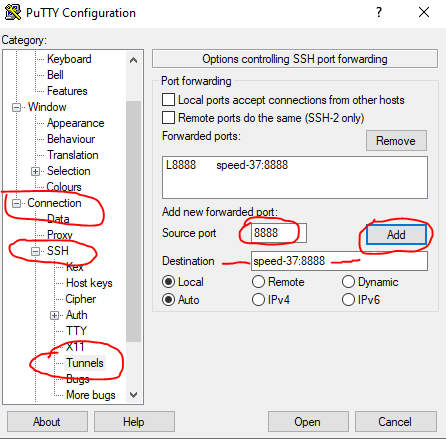
\includegraphics{images/putty1}}
	\caption{SSH tunnel configuration 1}
	\label{fig:putty1}
\end{figure}



\begin{figure}[htbp]
		\centering
		\fbox{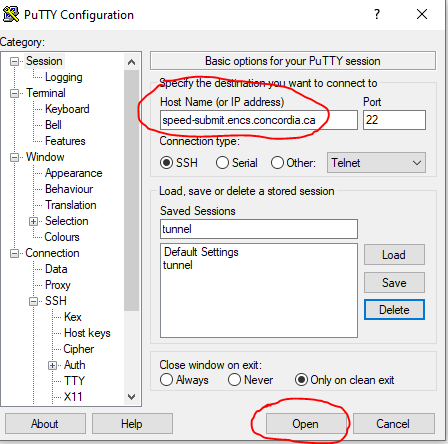
\includegraphics{images/putty2}}
	\caption{SSH tunnel configuration 2}
	\label{fig:putty2}
\end{figure}


\begin{figure}[htbp]
	\centering
	\fbox{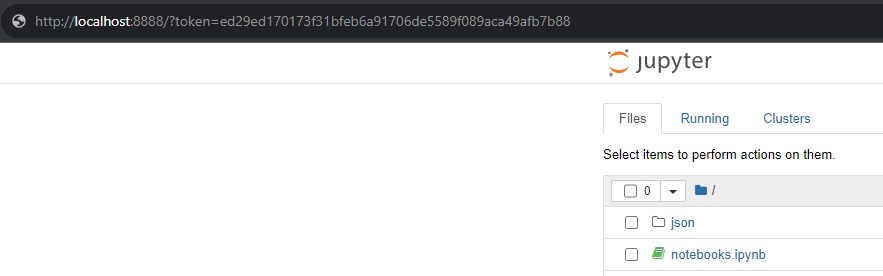
\includegraphics[width=1.00\textwidth]{images/jupyter.png}}
	\caption{Jupyter running on a Speed node}
	\label{fig:jupyter}
\end{figure}

% ------------------------------------------------------------------------------
\subsection{Scheduler Environment Variables}
\label{sect:env-vars}

The scheduler presents a number of environment variables that can be used in 
your jobs. You can invoke \tool{env} or \tool{printenv} in your
job to know what hose are (most begin with the prefix \texttt{SLURM}).
%
Some of the more useful ones are:
%\api{TMPDIR}, \api{SGE\_O\_WORKDIR}, and \api{NSLOTS}:

\begin{itemize}
\item
% TODO: verify temporal existence
\api{\$TMPDIR} -- the path to the job's temporary space on the node. It
\emph{only} exists for the duration of the job, so if data in the temporary space 
are important, they absolutely need to be accessed before the job terminates.

%\item
%\api{\$SGE\_O\_WORKDIR}=the path to the job's working directory (likely an
%NFS-mounted path). If, \texttt{-cwd}, was stipulated, that path is taken; if not, 
%the path defaults to your home directory.
\item
\api{\$SLURM\_SUBMIT\_DIR} -- the path to the job's working directory (likely an
NFS-mounted path). If, \option{--chdir}, was stipulated, that path is taken; if not, 
% TODO: verify if home or current:
the path defaults to your home directory.

% TODO: SLURM does not appear to have this
% SLURM_NTASKS
%\item
%\api{\$NSLOTS}=the number of cores requested for the job. This variable can 
%be used in place of hardcoded thread-request declarations. 

\item
\api{\$SLURM\_JOBID} -- your current jobs ID, useful for some manipulation
and reporting.

\item
\api{\$SLURM\_JOB\_NODELIST}=nodes participating in your job.

\item
\api{\$SLURM\_ARRAY\_TASK\_ID}=for array jobs (see \xs{sect:array-jobs}).

\item
See a more complete list here:

\small
\begin{itemize}
\item
\url{https://slurm.schedmd.com/srun.html#SECTION_INPUT-ENVIRONMENT-VARIABLES}
\item
\url{https://slurm.schedmd.com/srun.html#SECTION_OUTPUT-ENVIRONMENT-VARIABLES}
\end{itemize}
\normalsize

\end{itemize}

\noindent
In \xf{fig:tmpdir.sh} is a sample script, using some of these.

\begin{figure}[htpb]
    \lstinputlisting[language=csh,frame=single,basicstyle=\footnotesize\ttfamily]{tmpdir.sh}
    \caption{Source code for \file{tmpdir.sh}}
	\label{fig:tmpdir.sh}
\end{figure}


% ------------------------------------------------------------------------------
\subsection{SSH Keys For MPI}
\label{sect:ssh-mpi}

Some programs effect their parallel processing via MPI (which is a 
communication protocol). An example of such software is Fluent. MPI needs to 
have `passwordless login' set up, which means SSH keys. In your NFS-mounted 
home directory:

\begin{itemize}
\item
\texttt{cd .ssh}
\item
\texttt{ssh-keygen -t ed25519} (default location; blank passphrase) 
\item
\texttt{cat id\_ed25519.pub >> authorized\_keys} (if the \texttt{\href{https://www.ssh.com/academy/ssh/authorized-keys-file}{authorized\_keys}}
file already exists) \emph{OR} \texttt{cat id\_ed25519.pub > authorized\_keys} (if does not) 
\item
Set file permissions of \texttt{authorized\_keys} to 600; of your NFS-mounted home
to 700 (note that you likely will not have to do anything here, as most people
will have those permissions by default). 
\end{itemize}

% ------------------------------------------------------------------------------
\subsection{Creating Virtual Environments}
\label{sect:environments}
\label{sect:examples-venv}

The following documentation is specific to the \textbf{Speed} HPC Facility at the
Gina Cody School of Engineering and Computer Science.
%
Virtual environments typically instantiated via Conda or Python.
Another option is Singularity detailed in \xs{sect:singularity-containers}.
%
Usually, virtual environments are created once and before sending any job to the
scheduler, so when sending the job to the scheduler we (1) activate the virtual environment,
(2) use it, and (3) close it at the end of the job.


% ------------------------------------------------------------------------------
\subsubsection{Anaconda}
\label{sect:conda-venv}

To create an anaconda environment in your speed-scratch directory, use the \texttt{\-\-prefix} 
option when executing \texttt{conda create}. For example, to create an anaconda environment for 
\texttt{a\_user}, execute the following at the command line:

\begin{verbatim}
conda create --prefix /speed-scratch/a_user/myconda
\end{verbatim}

\vspace{10pt}
\noindent
\textbf{Note:} Without the \texttt{\-\-prefix} option, the \texttt{conda create} command creates the 
environment in \texttt{a\_user}'s home directory by default.
\vspace{10pt}

% ------------------------------------------------------------------------------
\paragraph{List Environments.}

To view your conda environments, type: \texttt{conda info --envs}

\begin{verbatim}
# conda environments:
#
base                  *  /encs/pkg/anaconda3-2019.07/root
                         /speed-scratch/a_user/myconda
\end{verbatim}      

% ------------------------------------------------------------------------------
\paragraph{Activate an Environment.}

Activate the environment \texttt{\/speed\-scratch\/a\_user\/myconda} as follows
\begin{verbatim}
conda activate /speed-scratch/a_user/myconda
\end{verbatim}
After activating your environment, add \tool{pip} to your environment by using 
\begin{verbatim}
conda install pip
\end{verbatim}
This will install \tool{pip} and \tool{pip}'s dependencies, including python, 
into the environment.

\begin{itemize}
	\item
		A consolidated example using Conda:
		\small
		\begin{verbatim}
			cd /speed-scratch/$USER
			srun --partition=p(s/g) -A Your_account --mem=10Gb --gpus=1 --pty /encs/bin/tcsh
			module load python/3.11.0/default
			conda create -p /speed-scratch/$USER/pytorch-env
			conda activate /speed-scratch/$USER/pytorch-env
			conda install python=3.11.0
			pip3 install torch torchvision torchaudio --index-url \ 
			  https://download.pytorch.org/whl/cu117
			....
			conda deactivate
			exit
		\end{verbatim}
		\normalsize
\end{itemize}

\noindent
\textbf{Important Note:} \tool{pip} (and \tool{pip3}) are used to install modules
from the python distribution while \texttt{conda install} installs modules from 
anaconda's repository.

% ------------------------------------------------------------------------------
\subsubsection{Python}
\label{sect:python-venv}

Setting up a Python virtual environment is fairly straightforward.
We have a simple example that use a Python virtual environment:

\begin{itemize}
	\item
		Using Python Venv
		\small
		\begin{verbatim}
			cd /speed-scratch/$USER
			srun --partition=p(s/g) -A Your_account --mem=10Gb --gpus=1 --pty /encs/bin/tcsh
			module load python/3.9.1/default
			mkdir -p /speed-scratch/$USER/tmp 
			setenv TMPDIR /speed-scratch/$USER/tmp
			setenv TMP /speed-scratch/$USER/tmp
			python -m venv $TMPDIR/testenv (testenv=name of the virtualEnv)
			source /speed-scratch/$USER/tmp/testenv/bin/activate.csh
			pip install modules…
			deactivate
			exit
		\end{verbatim}
		\normalsize
	\item
	    See, e.g., 
		\href
		{https://github.com/NAG-DevOps/speed-hpc/blob/master/src/gurobi-with-python.sh}
		{\texttt{gurobi-with-python.sh}}
\end{itemize}

\noindent
\textbf{Important Note:} partition \texttt{ps} is used for CPU jobs, partitions \texttt{pg}, \texttt{pt} are used
for GPU jobs, no need to use \texttt{--gpus=} when preparing environments for CPU jobs.

% ------------------------------------------------------------------------------
% TMP scheduler-specific section
% -------------- 2.12 Example Job Script: Fluent --------------
% -------------------------------------------------------------
\subsection{Example Job Script: Fluent}

\begin{figure}[htpb]
  \lstinputlisting[language=csh,frame=single,basicstyle=\footnotesize\ttfamily]{fluent.sh}
  \caption{Source code for \texttt{fluent.sh}}
  \label{fig:fluent.sh}
\end{figure}

The job script in \xf{fig:fluent.sh} runs Fluent in parallel over 32 cores. 
Notable aspects of this script include requesting e-mail notifications (\option{--mail-type}), 
defining the parallel environment for Fluent with \option{-t\$SLURM\_NTASKS} and \option{-g-cnf=\$FLUENTNODES}, 
and setting \api{\$TMPDIR} as the in-job location for the ``moment'' \file{rfile.out} file.
The script also copies everything from \api{\$TMPDIR} to a directory in the user's NFS-mounted home after the job completes.
Job progress can be monitored by examining the standard-out file (e.g.,
\texttt{slurm-249.out}), and/or by examining the ``moment'' file in TMPDIR (usually
\texttt{/disk/nobackup/<yourjob>} (it starts with your job-ID)) on the node running
the job. Be cautious with journal-file paths.

% -------------- 2.13 Example Job Script: EfficientDet --------
% -------------------------------------------------------------
\subsection{Example Job: EfficientDet}

The following steps describe how to create an EfficientDet environment on Speed, 
as submitted by a member of Dr. Amer's research group:

\begin{itemize}
  \item Navigate to your \texttt{speed-scratch} directory:
  \begin{verbatim}
	cd /speed-scratch/$USER
  \end{verbatim}
  \item Load Python module
  \begin{verbatim}
	module load python/3.8.3
  \end{verbatim}
  \item Create and activate the virtual environment
  \begin{verbatim}
	python3 -m venv <env_name>
	source <env_name>/bin/activate.csh
  \end{verbatim}
  \item Install DL packages for EfficientDet
  \small
  \begin{verbatim}
	pip install tensorflow==2.7.0
	pip install lxml>=4.6.1
	pip install absl-py>=0.10.0
	pip install matplotlib>=3.0.3
	pip install numpy>=1.19.4
	pip install Pillow>=6.0.0
	pip install PyYAML>=5.1
	pip install six>=1.15.0
	pip install tensorflow-addons>=0.12
	pip install tensorflow-hub>=0.11
	pip install neural-structured-learning>=1.3.1
	pip install tensorflow-model-optimization>=0.5
	pip install Cython>=0.29.13
	pip install git+https://github.com/cocodataset/cocoapi.git#subdirectory=PythonAPI
	\end{verbatim}
  \normalsize
\end{itemize}

% -------------- 2.14 Java Jobs -------------------------------
% -------------------------------------------------------------
\subsection{Java Jobs}
\label{sect:java}

Jobs that call Java have a memory overhead, which needs to be taken 
into account when assigning a value to \option{--mem}. Even the most basic 
Java call, such as \texttt{Java -Xmx1G -version}, will need to have,
\texttt{--mem=5G}, with the 4 GB difference representing the memory overhead. 
\textbf{Note} that this memory overhead grows proportionally with the value of
\texttt{-Xmx}. For example,

\begin{itemize}
  \item When \texttt{-Xmx} has a value of 100G, \option{--mem} has to be at least 106G.
  \item For \texttt{-Xmx} of 200G, \option{--mem} has to be at least 211G.
  \item For \texttt{-Xmx} of 300G, \option{--mem} has to be at least 314G.
\end{itemize}

% TODO: add MARF and GIPSY Java jobs

% -------------- 2.15 Scheduling on the GPU Nodes -------------
% -------------------------------------------------------------
\subsection{Scheduling on the GPU Nodes}
\label{sect:gpu-scheduling}

Speed has various GPU types in various subclusters of its nodes.

\begin{itemize}
	\item \texttt{speed-05} and \texttt{speed-17}:
The primary SPEED1 cluster has two GPU nodes, each with six Tesla (CUDA-compatible) P6
cards. Each card has 2048 cores and 16GB of RAM. Note that the P6
is mainly a single-precision card, so unless you need GPU double precision, 
double-precision calculations will be faster on a CPU node.
	\item \texttt{speed-01}:
This \texttt{vidpro} node (see \xf{fig:speed-architecture-full}, contact Dr.~Maria Amer) is identical
to 05 and 17 in its GPU configuration, but managed by the priority
for the vidpro group, that is a \texttt{pg} job scheduled there
is a subject for preemption.
	\item \texttt{speed-03}, \texttt{speed-25}, \texttt{speed-25}:
These \texttt{vidpro} nodes feature NVIDIA V100 cards with 32GB of RAM.
Like \texttt{speed-01}, the priority is of the vidpro group, who
purchased the nodes, and others' jobs are a subject from preemption
within \texttt{pg}, \texttt{pt}, and \texttt{cl} partitions.
	\item \texttt{speed-37}~--~\texttt{speed-43}:
SPEED2 nodes, the main backbone of the teaching partition \texttt{pt},
have 4x A100 80GB GPUs each, partitioned into average 4x MIGs of 20GB
each, with exceptions.
	\item \texttt{nebulae}:
A member of the Nebular subcluster (contact Dr.~Jun Yan), has 2x 48GB
RTX Ada 6000 cards. This node is in the \texttt{pn} partition.
	\item \texttt{speed-19}:
Has an AMD GPU, Tonga, 16GB of GPU ram.
This node along with the majority of the NVIDIA GPU nodes are in the
\texttt{cl} partition (with restrictions) to run OpenCL, Vulkan,
and HIP jobs.
\end{itemize}

\noindent
Job scripts for the GPU queues differ in that they need these statements,
which attach either a single GPU or more GPUs to the job with the
appropriate partition:
\begin{verbatim}
  #SBATCH --gpus=[1|x]
  #SBATCH -p [pg|pt|cl|pa]
\end{verbatim}
The default max quota for $x$ is 4.

\noindent
Once your job script is ready, submit it to the GPU partition (queue) with:
\begin{verbatim}
  sbatch --mem=<MEMORY> -p pg ./<myscript>.sh
\end{verbatim}
\option{--mem} and \option{-p} can reside in the script.

\noindent
You can query \tool{nvidia-smi} on the node \textbf{running your job} with:
\begin{verbatim}
  ssh <ENCSusername>@speed-[01|03|05|17|25|27|37-43]|nebulae nvidia-smi
\end{verbatim}

\noindent The status of the GPU queues can be queried e.g. with:
\begin{verbatim}
  sinfo -p pg --long --Node
  sinfo -p pt --long --Node
  sinfo -p cl --long --Node
  sinfo -p pa --long --Node
  sinfo -p pn --long --Node
\end{verbatim}

\noindent
You can query \tool{rocm-smi} on the AMD GPU node running your job with:
\begin{verbatim}
  ssh <ENCSusername>@speed-19 rocm-smi
\end{verbatim}

\noindent
\textbf{Important note for TensorFlow and PyTorch users}:
if you are planning to run TensorFlow and/or PyTorch multi-GPU jobs, please
\textbf{do not use} the \api{tf.distribute} and/or \api{torch.nn.DataParallel} functions 
on \textbf{speed-01, speed-05, or speed-17}, as they will crash the compute node (100\% certainty). 
This appears to be a defect in the current hardware architecture.
%
% TODO: Need to link to that example
The workaround is to either manually effect GPU parallelisation (see \xs{sect:multi-node-gpu})
(TensorFlow provides an example on how to do this), or to run on a single GPU,
which is now the default for those nodes.\\

\noindent \textbf{Important}:
Users without permission to use the GPU nodes can submit jobs to the various GPU
partitions, but those jobs will hang and never run.
Their availability can be seen with:
%
\small
\begin{verbatim}
[serguei@speed-submit src] % sinfo -p pg --long --Node
Thu Oct 19 22:31:04 2023
NODELIST   NODES PARTITION       STATE CPUS    S:C:T MEMORY TMP_DISK WEIGHT AVAIL_FE REASON
speed-05       1        pg        idle 32     2:16:1 515490        0      1    gpu16 none
speed-17       1        pg     drained 32     2:16:1 515490        0      1    gpu16 UGE
speed-25       1        pg        idle 32     2:16:1 257458        0      1    gpu32 none
speed-27       1        pg        idle 32     2:16:1 257458        0      1    gpu32 none
[serguei@speed-submit src] % sinfo -p pt --long --Node
Thu Oct 19 22:32:39 2023
NODELIST   NODES PARTITION       STATE CPUS    S:C:T MEMORY TMP_DISK WEIGHT AVAIL_FE REASON
speed-37       1        pt        idle 256    2:64:2 980275        0      1 gpu20,mi none
speed-38       1        pt        idle 256    2:64:2 980275        0      1 gpu20,mi none
speed-39       1        pt        idle 256    2:64:2 980275        0      1 gpu20,mi none
speed-40       1        pt        idle 256    2:64:2 980275        0      1 gpu20,mi none
speed-41       1        pt        idle 256    2:64:2 980275        0      1 gpu20,mi none
speed-42       1        pt        idle 256    2:64:2 980275        0      1 gpu20,mi none
speed-43       1        pt        idle 256    2:64:2 980275        0      1 gpu20,mi none
\end{verbatim}
\normalsize

\noindent
To specifically request a GPU node, add, \texttt{--gpus=[\#GPUs]},
to your \tool{sbatch} statement/script or \tool{salloc} statement request.
For example:
\begin{verbatim}
  sbatch -t 10 --mem=1G --gpus=1 -p pg ./tcsh.sh
\end{verbatim}
The request can be further specified to a specific node using \option{-w}
or a GPU type or feature.

\footnotesize
\begin{verbatim}
[serguei@speed-submit src] % squeue -p pg -o "%15N %.6D %7P %.11T %.4c %.8z %.6m %.8d %.6w %.8f %20G %20E"
NODELIST         NODES PARTITI       STATE MIN_    S:C:T MIN_ME MIN_TMP_  WCKEY FEATURES GROUP DEPENDENCY
speed-05             1 pg          RUNNING    1    *:*:*     1G        0 (null)   (null) 11929     (null)
[serguei@speed-submit src] % sinfo -p pg -o "%15N %.6D %7P %.11T %.4c %.8z %.6m %.8d %.6w %.8f %20G %20E"
NODELIST         NODES PARTITI       STATE CPUS    S:C:T MEMORY TMP_DISK WEIGHT AVAIL_FE GRES      REASON
speed-17             1 pg          drained   32   2:16:1 515490        0      1    gpu16 gpu:6        UGE
speed-05             1 pg            mixed   32   2:16:1 515490        0      1    gpu16 gpu:6       none
speed-[25,27]        2 pg             idle   32   2:16:1 257458        0      1    gpu32 gpu:2       none
\end{verbatim}
\normalsize

%  2.15.1 P6 on Multi-GPU, Multi-Node
% -------------------
\subsubsection{P6 on Multi-GPU, Multi-Node}
\label{sect:multi-node-gpu}

As described earlier, P6 cards are not compatible with \api{Distribute} and \api{DataParallel} functions
(\textbf{PyTorch}, \textbf{Tensorflow}) when running on multiple GPUs.
One workaround is to run the job in Multi-node, single GPU per node
(this applies to P6 nodes: speed-05, speed-17, speed-01):
\begin{verbatim}
  #SBATCH --nodes=2
  #SBATCH --gpus-per-node=1
\end{verbatim}

\noindent An example script for training on multiple nodes with multiple GPUs is provided in 
\href
  {https://github.com/NAG-DevOps/speed-hpc/blob/master/src/pytorch-multinode-multigpu.sh}
	{pytorch-multinode-multigpu.sh}
illustrates a job for training on Multi-Nodes, Multi-GPUs

%  2.15.2 CUDA
% -------------------
\subsubsection{CUDA}
\label{sect:cuda}

When calling \textbf{CUDA} within job scripts, it is important to link to the desired
the desired \textbf{CUDA} libraries and set the runtime link path to the same libraries. 
For example, to use the \texttt{cuda-11.5} libraries, specify the following in your \texttt{Makefile}.
\begin{verbatim}
  -L/encs/pkg/cuda-11.5/root/lib64 -Wl,-rpath,/encs/pkg/cuda-11.5/root/lib64
\end{verbatim}

\noindent In your job script, specify the version of \texttt{GCC} to use prior to calling CUDA:
\begin{verbatim}
  module load gcc/9.3
\end{verbatim}

%  2.15.3 Special Notes for Sending CUDA Jobs to the GPU Queue
% -------------------
\subsubsection{Special Notes for Sending CUDA Jobs to the GPU Queues}

Interactive jobs (\xs{sect:interactive-jobs}) must be submitted to the GPU partition to compile and link.
Several versions of CUDA are installed in:
\begin{verbatim}
  /encs/pkg/cuda-11.5/root/
  /encs/pkg/cuda-10.2/root/
  /encs/pkg/cuda-9.2/root
\end{verbatim}

\noindent For CUDA to compile properly for the GPU partition, edit your \texttt{Makefile}
replacing \texttt{\/usr\/local\/cuda} with one of the above.

%  2.15.4 OpenISS Examples
% -------------------
\subsubsection{OpenISS Examples}
\label{sect:openiss-examples}

These examples represent more comprehensive research-like jobs
for computer vision and other tasks with longer runtime (subject to the number of epochs and other parameters).
They derive from the actual research works of students and their theses and require the use of CUDA and GPUs.
These examples are available as ``native'' jobs on Speed and as Singularity containers.

\noindent Examples include:
\paragraph{OpenISS and REID}
\label{sect:openiss-reid}

A computer-vision-based person re-identification 
(e.g., motion capture-based tracking for stage performance) part of the OpenISS
project by Haotao Lai~\cite{lai-haotao-mcthesis19} using TensorFlow and Keras.
The script is available here:
\href{https://github.com/NAG-DevOps/speed-hpc/blob/master/src/openiss-reid-speed.sh}{openiss-reid-speed.sh}.
The fork of the original repo~\cite{openiss-reid-tfk} adjusted to run on Speed is available here:
\href{https://github.com/NAG-DevOps/openiss-reid-tfk}{openiss-reid-tfk}.
Detailed instructions on how to run it on Speed are in the README:
\url{https://github.com/NAG-DevOps/speed-hpc/tree/master/src#openiss-reid-tfk}

\paragraph{OpenISS and YOLOv3}
\label{sect:openiss-yolov3}

The related code using YOLOv3 framework is in the
the fork of the original repo~\cite{openiss-yolov3} adjusted
to to run on Speed is available here: \href{https://github.com/NAG-DevOps/openiss-yolov3}{openiss-yolov3}.\\

\noindent Example job scripts can run on both CPUs and GPUs, as well as interactively using TensorFlow:

\begin{itemize}
	\item Interactive mode:
  \href{https://github.com/NAG-DevOps/speed-hpc/blob/master/src/openiss-yolo-interactive.sh}
  {openiss-yolo-interactive.sh}
	\item CPU-based job:
  \href{https://github.com/NAG-DevOps/speed-hpc/blob/master/src/openiss-yolo-cpu.sh}
  {openiss-yolo-cpu.sh}
	\item GPU-based job:
  \href{https://github.com/NAG-DevOps/speed-hpc/blob/master/src/openiss-yolo-gpu.sh}
  {openiss-yolo-gpu.sh}
\end{itemize}

\noindent Detailed instructions on how to run these on Speed are in the README: 
\url{https://github.com/NAG-DevOps/speed-hpc/tree/master/src#openiss-yolov3}

% -------------- 2.16 Singularity Containers ------------------
% -------------------------------------------------------------
\subsection{Singularity Containers}
\label{sect:singularity-containers}

Singularity is a container platform designed to execute applications in a portable, 
reproducible, and secure manner. Unlike Docker, Singularity does not require root privileges, 
making it more suitable for HPC environments. If the \tool{/encs} software tree does not have 
the required software available, another option is to run Singularity containers. 
We run EL7 and EL9 flavors of Linux, and if some projects require Ubuntu or 
other distributions, it is possible to run that software as a container, 
including those converted from Docker. The currently recommended version of Singularity 
is \texttt{singularity/3.10.4/default}.\\

The example
\href{https://github.com/NAG-DevOps/speed-hpc/blob/master/src/lambdal-singularity.sh}{lambdal-singularity.sh}
showcases an immediate use of a container built for the Ubuntu-based LambdaLabs software stack, 
originally built as a Docker image then pulled in as a Singularity container. The source material
used for the docker image was our fork of their official repository: 
\url{https://github.com/NAG-DevOps/lambda-stack-dockerfiles}.\\

\noindent \textbf{Note}: If you make your own containers or pull from DockerHub,
use your \verb+/speed-scratch/$USER+ directory, as these images may easily 
consume gigabytes of space in your home directory, quickly exhausting your quota.\\

\noindent \textbf{Tip}: To check your quota and find big files, 
see \xs{sect:quota-exceeded} and
\href{https://www.concordia.ca/ginacody/aits/encs-data-storage.html}{ENCS Data Storage}.\\

We have also built equivalent OpenISS (\xs{sect:openiss-examples}) containers from their Docker 
counterparts for teaching and research purposes~\cite{oi-containers-poster-siggraph2023}. 
The images from \url{https://github.com/NAG-DevOps/openiss-dockerfiles}
and their DockerHub equivalents \url{https://hub.docker.com/u/openiss} can be found in 
\verb+/speed-scratch/nag-public+ with a `\texttt{.sif}' extension.
Some can be run in both batch and interactive modes, covering basics with CUDA, OpenGL rendering, 
and computer vision tasks. Examples include Jupyter notebooks with Conda support.

\begin{verbatim}
  /speed-scratch/nag-public:
  openiss-cuda-conda-jupyter.sif
  openiss-cuda-devicequery.sif
  openiss-opengl-base.sif
  openiss-opengl-cubes.sif
  openiss-opengl-triangle.sif
  openiss-reid.sif
  openiss-xeyes.sif
\end{verbatim}

This section introduces working with Singularity, its containers, and what can and cannot 
be done with Singularity on the ENCS infrastructure. For comprehensive documentation, 
refer to the authors' guide: \url{https://www.sylabs.io/docs/}.\\

Singularity containers are either built from an existing container, or from scratch. 
Building from scratch requires a recipe file (think of like a Dockerfile) and
must be done with root permissions, which are not available on the ENCS infrastructure. 
Therefore, built-from-scratch containers must be created on a user-managed/personal system. 
There are three types of Singularity containers:
% with one exception (see, Building A Container From An Existing Container).

\begin{itemize}
  \item File-system containers: built around the ext3 file system and are read-write ``file'', but cannot be resized once built.
  \item Sandbox containers: essentially a directory in an existing read-write space and are also read-write.
  \item Squashfs containers: read-only compressed ``file'' and are read-only. It is the default build type.
\end{itemize}

\noindent
``A common workflow is to use the ``sandbox'' mode for container development and then build it as a 
default (squashfs) Singularity image when done.'' says the Singularity's authors about builds.
File-system containers are considered legacy and are not commonly used.\\

For many workflows, a Docker container might already exist. In this case, you can use Singularity's 
docker pull function as part of your virtual environment setup in an interactive job allocation:

\small
\begin{verbatim}
  salloc --gpus=1 -n8 --mem=4Gb -t60
  cd /speed-scratch/$USER/
  singularity pull openiss-cuda-devicequery.sif docker://openiss/openiss-cuda-devicequery
  INFO:    Converting OCI blobs to SIF format
  INFO:    Starting build...
\end{verbatim}
\normalsize

\noindent
This method can be used for converting Docker containers directly on Speed.
On GPU nodes, make sure to pass on the \option{--nv} flag to Singularity so its containers 
could access the GPUs. See the linked example for more details.


% ------------------------------------------------------------------------------
\section{Conclusion}
\label{sect:conclusion}

The cluster is, ``first come, first served'', until it fills, and then job
position in the queue is based upon past usage. The scheduler does attempt
to fill gaps, though, so sometimes a single-core job of lower priority
will schedule before a multi-core job of higher priority, for example.

% ------------------------------------------------------------------------------
\subsection{Important Limitations}
\label{sect:limitations}

\begin{itemize}
\item
New users are restricted to a total of 32 cores: write to \url{rt-ex-hpc@encs.concordia.ca}
if you need more temporarily (192 is the maximum, or, 6 jobs of 32 cores each).

\item
Batch job sessions are a maximum of one week in length (only 24 hours, though,
for interactive jobs, see \xs{sect:interactive-jobs}).

\item
Scripts can live in your NFS-provided home, but any substantial data need
to be in your cluster-specific directory
(located at \verb+/speed-scratch/<ENCSusername>/+).

NFS is great for acute activity, but is not ideal for chronic activity.
Any data that a job will 
read more than once should be copied at the start to the scratch disk of a 
compute node using \api{\$TMPDIR} (and, perhaps, \api{\$SLURM\_SUBMIT\_DIR}), 
any intermediary job data should be produced in \api{\$TMPDIR}, and once a 
job is near to finishing, those data should be copied to your NFS-mounted 
home (or other NFS-mounted space) from \api{\$TMPDIR} (to, perhaps,
\api{\$SLURM\_SUBMIT\_DIR}). In other words, IO-intensive operations should be effected 
locally whenever possible, saving network activity for the start and end of 
jobs. 

\item
Your current resource allocation is based upon past usage, which is an 
amalgamation of approximately one week's worth of past wallclock (i.e., time 
spent on the node(s)) and compute activity (on the node(s)).

\item
Jobs should NEVER be run outside of the province of the scheduler.
Repeat offenders risk loss of cluster access. 

\end{itemize}

% ------------------------------------------------------------------------------
% TMP scheduler-specific section
% ------------------------------------------------------------------------------
\subsection{Tips/Tricks}
\label{sect:tips}

\begin{itemize}
\item
Files/scripts must have Linux line breaks in them (not Windows ones).
Use \tool{file} command to verify; and \tool{dos2unix} command
to convert.

\item
Use \tool{rsync}, not \tool{scp}, when moving a lot of data around.

\item
If you are going to move many many files between NFS-mounted storage and the 
cluster, \tool{tar} everything up first. 

\item
If you intend to use a different shell (e.g., \tool{bash}~\cite{aosa-book-vol1-bash}),
%you will need to source a different scheduler file, and
you will need to change the shell declaration in your script(s).

% TODO:
%\item
%The load displayed in \tool{qstat} by default is \api{np\_load}, which is
%load/\#cores. That means that a load of, ``1'', which represents a fully active 
%core, is displayed as $0.03$ on the node in question, as there are 32 cores 
%on a node. To display load ``as is'' (such that a node with a fully active 
%core displays a load of approximately $1.00$), add the following to your
%\file{.tcshrc} file: \texttt{setenv SGE\_LOAD\_AVG load\_avg}

\item
\textbf{Try to request resources that closely match what your job will use: 
requesting many more cores or much more memory than will be needed makes a 
job more difficult to schedule when resources are scarce.}

\item
E-mail, \texttt{rt-ex-hpc AT encs.concordia.ca}, with any concerns/questions.
\end{itemize}


% ------------------------------------------------------------------------------
\subsection{Use Cases}
\label{sect:cases}

\begin{itemize}
	\item 
HPC Committee's initial batch about 6 students (end of 2019):
\begin{itemize}
	\item 
10000 iterations job in Fluent finished in $<26$ hours vs. 46 hours in Calcul Quebec
\end{itemize}
	\item 
NAG's MAC spoofer analyzer~\cite{mac-spoofer-analyzer-intro-c3s2e2014,mac-spoofer-analyzer-detail-fps2014},
such as \url{https://github.com/smokhov/atsm/tree/master/examples/flucid}
\begin{itemize}
	\item 
compilation of forensic computing reasoning cases about false or true positives of hardware address spoofing in the labs
\end{itemize}
	\item 
S4 LAB/GIPSY R\&D Group's:
\begin{itemize}
	\item 
MARFCAT and MARFPCAT (OSS signal processing and machine learning tools for 
vulnerable and weak code analysis and network packet capture
analysis)~\cite{marfcat-nlp-ai2014,marfcat-sate2010-nist,fingerprinting-mal-traffic}
	\item 
Web service data conversion and analysis
	\item 
{\flucid} encoders (translation of large log data into {\flucid}~\cite{mokhov-phd-thesis-2013} for forensic analysis)
	\item 
Genomic alignment exercises
\end{itemize}
\item
\bibentry{oi-containers-poster-siggraph2023}
\item
\bibentry{Gopal2024Sep}
\item
\bibentry{Gopal2023Mob}
\item
\bibentry{cfd-modeling-turbine-2023}
\item
\bibentry{cfd-vaxis-turbine-wake-2022}
\item
\bibentry{numerical-turbulence-vawt-2021}
\item
\bibentry{niksirat2020}

\item
The work ``\bibentry{lai-haotao-mcthesis19}'' using TensorFlow and Keras on OpenISS
adjusted to run on Speed based on the repositories:
\begin{itemize}
	\item 
\bibentry{openiss-reid-tfk} and
	\item
\bibentry{openiss-yolov3}
\end{itemize}
and theirs forks by the team.

\end{itemize}

% ------------------------------------------------------------------------------
\appendix

% ------------------------------------------------------------------------------
\section{History}

% ------------------------------------------------------------------------------
\subsection{Acknowledgments}
\label{sect:acks}

\begin{itemize}
	\item 
The first 6 (to 6.5) versions of this manual and early UGE job script samples,
Singularity testing and user support were produced/done by Dr.~Scott Bunnell
during his time at Concordia as a part of the NAG/HPC group. We thank
him for his contributions.
	\item 
The HTML version with devcontainer support was contributed by Anh H Nguyen.
	\item 
Dr.~Tariq Daradkeh, was our IT Instructional Specialist August 2022 to September 2023;
working on the scheduler, scheduling research, end user support, and integration of
examples, such as YOLOv3 in \xs{sect:openiss-yolov3} other tasks. We have a continued
collaboration on HPC/scheduling research.
\end{itemize}

% ------------------------------------------------------------------------------
\subsection{Migration from UGE to SLURM}
\label{appdx:uge-to-slurm}

For long term users who started off with Grid Engine here are some resources
to make a transition and mapping to the job submission process.

\begin{itemize}
\item
Queues are called ``partitions'' in SLURM. Our mapping from the GE queues
to SLURM partitions is as follows:
\begin{verbatim}
GE  => SLURM
s.q    ps
g.q    pg
a.q    pa
\end{verbatim}
We also have a new partition \texttt{pt} that covers SPEED2 nodes,
which previously did not exist.

\item
Commands and command options mappings are found in \xf{fig:rosetta-mappings} from\\
\url{https://slurm.schedmd.com/rosetta.pdf}\\
\url{https://slurm.schedmd.com/pdfs/summary.pdf}\\
Other related helpful resources from similar organizations who either used
SLURM for awhile or also transitioned to it:\\
\small
\url{https://docs.alliancecan.ca/wiki/Running_jobs}\\
\url{https://www.depts.ttu.edu/hpcc/userguides/general_guides/Conversion_Table_1.pdf}\\
\url{https://docs.mpcdf.mpg.de/doc/computing/clusters/aux/migration-from-sge-to-slurm}
\normalsize

\begin{figure}[htpb]
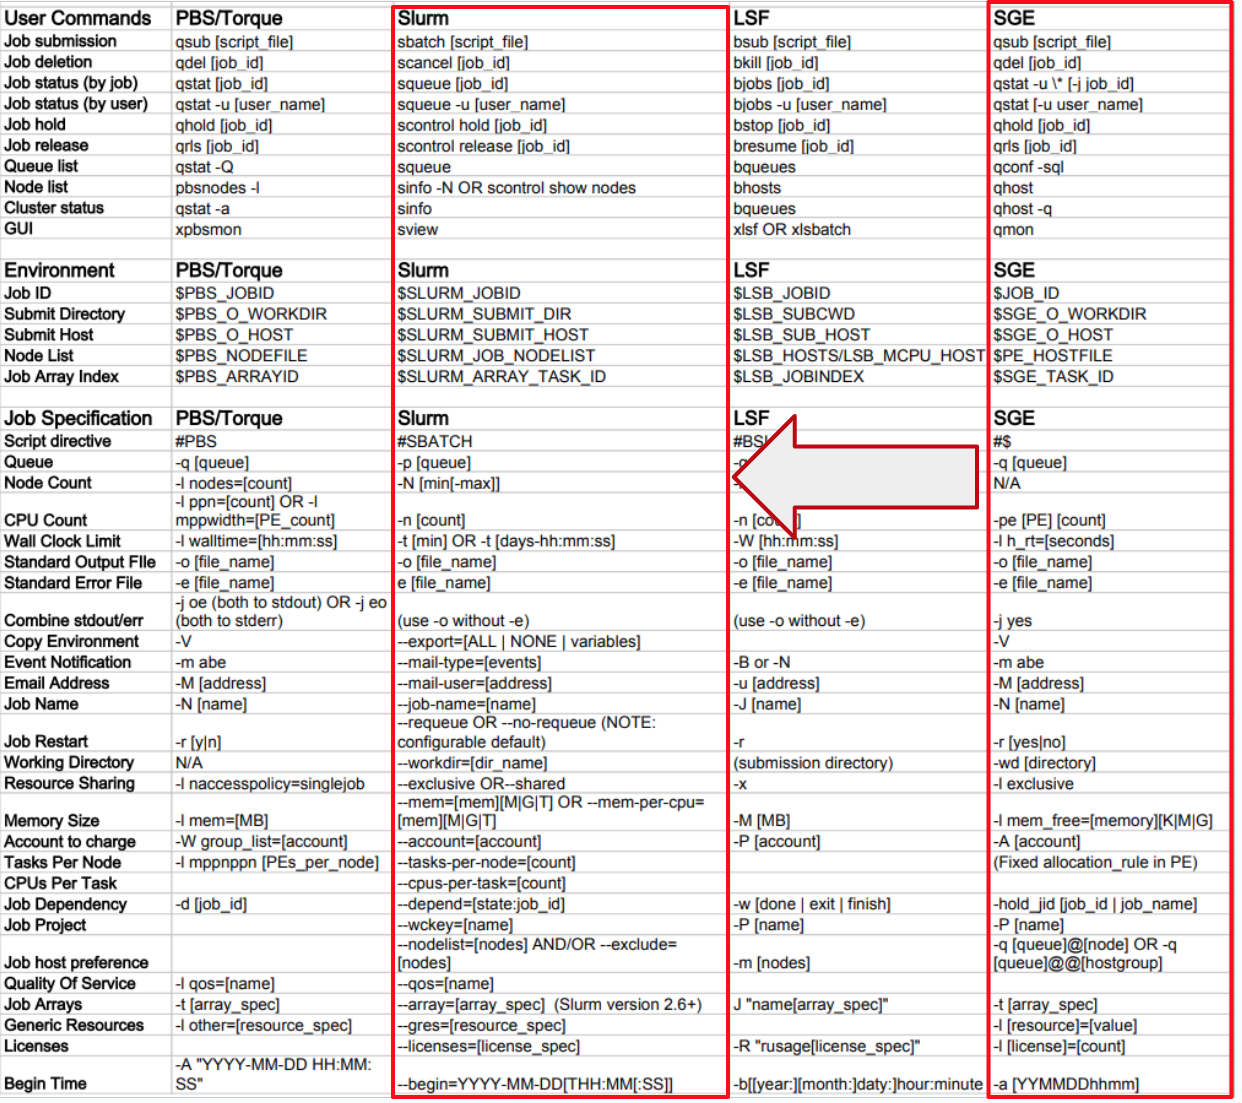
\includegraphics[width=\columnwidth]{images/rosetta-mapping}
\caption{Rosetta Mappings of Scheduler Commands from SchedMD}
\label{fig:rosetta-mappings}
\end{figure}

\item
\noindent
\textbf{NOTE:} If you have used UGE commands in the past you probably still have these
lines there; \textbf{they should now be removed}, as they have no use in SLURM and
will start giving ``command not found'' errors on login when the software is removed:

csh/\tool{tcsh}:
Sample \file{.tcshrc} file:
\begin{verbatim}
# Speed environment set up 
if ($HOSTNAME == speed-submit.encs.concordia.ca) then
   source /local/pkg/uge-8.6.3/root/default/common/settings.csh
endif
\end{verbatim}

Bourne shell/\tool{bash}:
Sample \file{.bashrc} file:
\begin{verbatim}
# Speed environment set up 
if [ $HOSTNAME = "speed-submit.encs.concordia.ca" ]; then
    . /local/pkg/uge-8.6.3/root/default/common/settings.sh
    printenv ORGANIZATION | grep -qw ENCS || . /encs/Share/bash/profile
fi
\end{verbatim}

Note that you will need to either log out and back in, or execute a new shell, 
for the environment changes in the updated \file{.tcshrc} or \file{.bashrc} file to be applied 
(\textbf{important}).


\end{itemize}

% ------------------------------------------------------------------------------
\subsection{Phases}
\label{sect:phases}

Brief summary of Speed evolution phases.

% ------------------------------------------------------------------------------
\subsubsection{Phase 4}

Phase 4 had 7 SuperMicro servers with 4x A100 80GB GPUs each added,
dubbed as ``SPEED2''. We also moved from Grid Engine to SLURM.

% ------------------------------------------------------------------------------
\subsubsection{Phase 3}

Phase 3 had 4 vidpro nodes added from Dr.~Amer totalling 6x P6 and 6x V100
GPUs added.

% ------------------------------------------------------------------------------
\subsubsection{Phase 2}

Phase 2 saw 6x NVIDIA Tesla P6 added and 8x more compute nodes.
The P6s replaced 4x of FirePro S7150.

% ------------------------------------------------------------------------------
\subsubsection{Phase 1}

Phase 1 of Speed was of the following configuration:

\begin{itemize}
\item
Sixteen, 32-core nodes, each with 512~GB of memory and approximately 1~TB of volatile-scratch disk space. 
\item
Five AMD FirePro S7150 GPUs, with 8~GB of memory (compatible with the Direct X, OpenGL, OpenCL, and Vulkan APIs). 
\end{itemize}

% ------------------------------------------------------------------------------
% TMP scheduler-specific section
% ------------------------------------------------------------------------------
%						B Frequently Asked Questions 
% ------------------------------------------------------------------------------
\section{Frequently Asked Questions}
\label{sect:faqs}

% B.1 Where do I learn about Linux?
% -------------------------------------------------------------
\subsection{Where do I learn about Linux?}
\label{sect:faqs-linux}

All Speed users are expected to have a basic understanding of Linux and its commonly used commands.
Here are some recommended resources:

\paragraph*{Software Carpentry}
Software Carpentry provides free resources to learn software, including a workshop on the Unix shell.
Visit \href{https://software-carpentry.org/lessons/}{Software Carpentry Lessons} to learn more.

\paragraph*{Udemy}
There are numerous Udemy courses, including free ones, that will help you learn Linux. 
Active Concordia faculty, staff and students have access to Udemy courses. 
A recommended starting point for beginners is the course ``Linux Mastery: Master the Linux Command Line in 11.5 Hours''.
Visit \href{https://www.concordia.ca/it/services/udemy.html}{Concordia's Udemy page} to learn how Concordians can access Udemy.

% B.2 How to bash shell on Speed?
% -------------------------------------------------------------
\subsection{How to use bash shell on \tool{Speed}?}
\label{sect:faqs-bash}

This section provides comprehensive instructions on how to utilize the bash shell on the Speed cluster.

% B.2.1 How do I set bash as my login shell?
\subsubsection{How do I set bash as my login shell?}
To set your default login shell to bash on Speed, your login shell on all GCS servers must be changed to bash.
To make this change, create a ticket with the Service Desk (or email \texttt{help at concordia.ca}) to
request that bash become your default login shell for your ENCS user account on all GCS servers.

% B.2.2 How do I move into a bash shell on Speed?
\subsubsection{How do I move into a bash shell on \tool{Speed}?}
To move to the bash shell, type \textbf{bash} at the command prompt:
\begin{verbatim}
	[speed-submit] [/home/a/a_user] > bash
	bash-4.4$ echo $0
	bash
\end{verbatim}	

\noindent \textbf{Note} how the command prompt changes from 
``\verb![speed-submit] [/home/a/a_user] >!'' to ``\verb!bash-4.4$!'' after entering the bash shell.

% B.2.3 How do I use the bash shell in an interactive session on Speed?
\subsubsection{How do I use the bash shell in an interactive session on \tool{Speed}?}
Below are examples of how to use \tool{bash} as a shell in your interactive job sessions 
with both the \tool{salloc} and \tool{srun} commands.

\begin{itemize}
	\item \texttt{salloc -ppt --mem=100G -N 1 -n 10 /encs/bin/bash}
	\item \texttt{srun  --mem=50G -n 5 --pty /encs/bin/bash}
\end{itemize}

\noindent\textbf{Note:} Make sure the interactive job requests memory, cores, etc.

% B.2.4 How do I run scripts written in bash on Speed?
\subsubsection{How do I run scripts written in bash on \tool{Speed}?}

To execute bash scripts on Speed:
\begin{enumerate}
	\item Ensure that the shebang of your bash job script is \verb+#!/encs/bin/bash+
	\item Use the \tool{sbatch} command to submit your job script to the scheduler.
\end{enumerate}

\noindent Check Speed GitHub for a 
\href{https://github.com/NAG-DevOps/speed-hpc/blob/master/src/bash.sh}{sample bash job script}.

% B.3 How to resolve “Disk quota exceeded” errors?
% -------------------------------------------------------------
\subsection{How to resolve ``Disk quota exceeded'' errors?}

% B.3.1 Probable Cause
\subsubsection{Probable Cause}

The ``\texttt{Disk quota exceeded}'' error occurs when your application has 
run out of disk space to write to. On \tool{Speed}, this error can be returned when:
\begin{enumerate}
	\item The NFS-provided home is full and cannot be written to.
	You can verify this using the \tool{quota} and \tool{bigfiles} commands.
	\item The ``\texttt{/tmp}'' directory on the speed node where your application is running is full and cannot be written to.
\end{enumerate}

% B.3.2 Possible Solutions
\subsubsection{Possible Solutions}

\begin{enumerate}
	\item Use the \option{--chdir} job script option to set the job working directory.
	This is the directory where the job will write output files.

 	\item Although local disk space is recommended for IO-intensive operations, the 
 	`\texttt{/tmp}' directory on \tool{Speed} nodes is limited to 1TB, so it may be necessary 
	to store temporary data elsewhere. Review the documentation for each module
	used in your script to determine how to set working directories.
	The basic steps are:
	\begin{itemize}
		\item
		Determine how to set working directories for each module used in your job script.
		\item
		Create a working directory in \tool{speed-scratch} for output files:
		\begin{verbatim}
			mkdir -m 750 /speed-scratch/$USER/output
		\end{verbatim}
		\item
		Create a subdirectory for recovery files:
		\begin{verbatim}
			mkdir -m 750 /speed-scratch/$USER/recovery
		\end{verbatim}
		\item
		Update the job script to write output to the directories created in your 
		\tool{speed-scratch} directory, e.g., \verb!/speed-scratch/$USER/output!.
	\end{itemize}
\end{enumerate}
\noindent In the above example, \verb!$USER! is an environment variable containing your ENCS username.

% B.3.3 Example of setting working directories for COMSOL
\subsubsection{Example of setting working directories for \tool{COMSOL}}

\begin{itemize}
	\item Create directories for recovery, temporary, and configuration files. 
	\begin{verbatim}
		mkdir -m 750 -p /speed-scratch/$USER/comsol/{recovery,tmp,config}
	\end{verbatim}
	\item Add the following command switches to the COMSOL command to use the 
	directories created above:
	\begin{verbatim} 
		-recoverydir /speed-scratch/$USER/comsol/recovery 
		-tmpdir /speed-scratch/$USER/comsol/tmp
		-configuration/speed-scratch/$USER/comsol/config
	\end{verbatim}
\end{itemize} 
\noindent In the above example, \verb!$USER! is an environment variable containing your ENCS username.

% B.3.4 Example of setting working directories for Python Modules
\subsubsection{Example of setting working directories for \tool{Python Modules}}

By default when adding a Python module, the \texttt{/tmp} directory is set as the temporary repository for files downloads.
The size of the \texttt{/tmp} directory on \verb!speed-submit! is too small for PyTorch.
To add a Python module
\begin{itemize}
    \item Create your own tmp directory in your \verb!speed-scratch! directory:
	\begin{verbatim} 
  		mkdir /speed-scratch/$USER/tmp
	\end{verbatim}
	\item Use the temporary directory you created
	\begin{verbatim} 
  		setenv TMPDIR /speed-scratch/$USER/tmp
	\end{verbatim}
    \item Attempt the installation of PyTorch
\end{itemize}
\noindent In the above example, \verb!$USER! is an environment variable containing your ENCS username.

% B.4 How do I check my job's status?
% -------------------------------------------------------------
\subsection{How do I check my job's status?}

%When a job with a job id of 1234 is running, the status of that job can be tracked using \verb!`qstat -j 1234`!.
%Likewise, if the job is pending, the \verb!`qstat -j 1234`! command will report as to why the job is not scheduled or running.
%Once the job has finished, or has been killed, the \textbf{qacct} command must be used to query the job's status, e.g., \verb!`qaact -j [jobid]`!. 
When a job with a job ID of 1234 is running or terminated, 
you can track its status using the following commands:
\begin{itemize}
	\item Use the ``sacct'' command to view the status of a job:
	\begin{verbatim} 
		sacct -j 1234
	\end{verbatim}
	\item Use the ``squeue'' command to see if the job is sitting in the queue:
	\begin{verbatim} 
		squeue -j 1234
	\end{verbatim}
	\item Use the ``sstat'' command to find long-term statistics on the job after it has terminated 
	and the \tool{slurmctld} has purged it from its tracking state into the database:
	\begin{verbatim} 
		sstat -j 1234
	\end{verbatim}
\end{itemize}

% B.5 Why is my job pending when nodes are empty?
% -------------------------------------------------------------
\subsection{Why is my job pending when nodes are empty?}

% B.5.1 Disabled nodes
\subsubsection{Disabled nodes}
It is possible that one or more of the Speed nodes are disabled for maintenance.
To verify if Speed nodes are disabled, check if they are in a draining or drained state:

%\begin{verbatim}
%qstat -f -qs d
%queuename                      qtype resv/used/tot. load_avg arch          states
%---------------------------------------------------------------------------------
%g.q@speed-05.encs.concordia.ca BIP   0/0/32         0.27     lx-amd64      d
%---------------------------------------------------------------------------------
%s.q@speed-07.encs.concordia.ca BIP   0/0/32         0.01     lx-amd64      d
%---------------------------------------------------------------------------------
%s.q@speed-10.encs.concordia.ca BIP   0/0/32         0.01     lx-amd64      d
%---------------------------------------------------------------------------------
%s.q@speed-16.encs.concordia.ca BIP   0/0/32         0.02     lx-amd64      d
%---------------------------------------------------------------------------------
%s.q@speed-19.encs.concordia.ca BIP   0/0/32         0.03     lx-amd64      d
%---------------------------------------------------------------------------------
%s.q@speed-24.encs.concordia.ca BIP   0/0/32         0.01     lx-amd64      d
%---------------------------------------------------------------------------------
%s.q@speed-36.encs.concordia.ca BIP   0/0/32         0.03     lx-amd64      d
%\end{verbatim}

\small
\begin{verbatim}
[serguei@speed-submit src] % sinfo --long --Node
Thu Oct 19 21:25:12 2023
NODELIST   NODES PARTITION       STATE CPUS    S:C:T MEMORY TMP_DISK WEIGHT AVAIL_FE REASON
speed-01       1        pa        idle 32     2:16:1 257458        0      1    gpu16 none
speed-03       1        pa        idle 32     2:16:1 257458        0      1    gpu32 none
speed-05       1        pg        idle 32     2:16:1 515490        0      1    gpu16 none
speed-07       1       ps*       mixed 32     2:16:1 515490        0      1    cpu32 none
speed-08       1       ps*     drained 32     2:16:1 515490        0      1    cpu32 UGE
speed-09       1       ps*     drained 32     2:16:1 515490        0      1    cpu32 UGE
speed-10       1       ps*     drained 32     2:16:1 515490        0      1    cpu32 UGE
speed-11       1       ps*        idle 32     2:16:1 515490        0      1    cpu32 none
speed-12       1       ps*     drained 32     2:16:1 515490        0      1    cpu32 UGE
speed-15       1       ps*     drained 32     2:16:1 515490        0      1    cpu32 UGE
speed-16       1       ps*     drained 32     2:16:1 515490        0      1    cpu32 UGE
speed-17       1        pg     drained 32     2:16:1 515490        0      1    gpu16 UGE
speed-19       1       ps*        idle 32     2:16:1 515490        0      1    cpu32 none
speed-20       1       ps*     drained 32     2:16:1 515490        0      1    cpu32 UGE
speed-21       1       ps*     drained 32     2:16:1 515490        0      1    cpu32 UGE
speed-22       1       ps*     drained 32     2:16:1 515490        0      1    cpu32 UGE
speed-23       1       ps*        idle 32     2:16:1 515490        0      1    cpu32 none
speed-24       1       ps*        idle 32     2:16:1 515490        0      1    cpu32 none
speed-25       1        pg        idle 32     2:16:1 257458        0      1    gpu32 none
speed-25       1        pa        idle 32     2:16:1 257458        0      1    gpu32 none
speed-27       1        pg        idle 32     2:16:1 257458        0      1    gpu32 none
speed-27       1        pa        idle 32     2:16:1 257458        0      1    gpu32 none
speed-29       1       ps*        idle 32     2:16:1 515490        0      1    cpu32 none
speed-30       1       ps*     drained 32     2:16:1 515490        0      1    cpu32 UGE
speed-31       1       ps*     drained 32     2:16:1 515490        0      1    cpu32 UGE
speed-32       1       ps*     drained 32     2:16:1 515490        0      1    cpu32 UGE
speed-33       1       ps*        idle 32     2:16:1 515490        0      1    cpu32 none
speed-34       1       ps*        idle 32     2:16:1 515490        0      1    cpu32 none
speed-35       1       ps*     drained 32     2:16:1 515490        0      1    cpu32 UGE
speed-36       1       ps*     drained 32     2:16:1 515490        0      1    cpu32 UGE
speed-37       1        pt        idle 256    2:64:2 980275        0      1 gpu20,mi none
speed-38       1        pt        idle 256    2:64:2 980275        0      1 gpu20,mi none
speed-39       1        pt        idle 256    2:64:2 980275        0      1 gpu20,mi none
speed-40       1        pt        idle 256    2:64:2 980275        0      1 gpu20,mi none
speed-41       1        pt        idle 256    2:64:2 980275        0      1 gpu20,mi none
speed-42       1        pt        idle 256    2:64:2 980275        0      1 gpu20,mi none
speed-43       1        pt        idle 256    2:64:2 980275        0      1 gpu20,mi none
\end{verbatim}
\normalsize

\noindent Note which nodes are in the state of \textbf{drained}.
The reason for the drained state can be found in the \textbf{reason} column.\\

\noindent Your job will run once an occupied node becomes availble or the maintenance is completed, 
and the disabled nodes have a state of \textbf{idle}.

% B.5.2 Error in job submit request.
\subsubsection{Error in job submit request.}

It is possible that your job is pending because it requested resources that are not available within Speed. 
To verify why job ID 1234 is not running, execute:
\begin{verbatim} 
	sacct -j 1234
\end{verbatim}

\noindent A summary of the reasons can be obtained via the \tool{squeue} command.
%and review the messages in the \textbf{scheduling info:} section.


% ------------------------------------------------------------------------------
\section{Sister Facilities}

Below is a list of resources and facilities similar to Speed at various capacities.
Depending on your research group and needs, they might be available to you. They
are not managed by HPC/NAG of AITS, so contact their respective representatives.

\begin{itemize}
\item
\texttt{computation.encs} CPU only 3-machine cluster running longer jobs
without a scheduler at the moment
\item
\texttt{apini.encs} cluster for teaching and MPI programming (see the corresponding
course in CSSE)
\item
Computer Science and Software Engineering (CSSE) Virya GPU Cluster. For CSSE 
members only. The cluster has 4 nodes with total of 32 NVIDIA GPUs (a mix of
V100s and A100s). To request access send email to \texttt{virya.help@concordia.ca}.
\item
Dr. Maria Amer's VidPro group's nodes in Speed (-01, -03, -25, -27) with additional V100 and P6 GPUs.
\item
There are various Lambda Labs other GPU servers and like computers
acquired by individual researchers; if you are member of their
research group, contact them directly. These resources are not
managed by us.
\begin{itemize}
\item
Dr. Amin Hammad's \texttt{construction.encs} Lambda Labs station
\item
Dr. Hassan Rivaz's \texttt{impactlab.encs} Lambda Labs station
\item
Dr. Nizar Bouguila's \texttt{xailab.encs} Lambda Labs station
\item
Dr. Roch Glitho's \texttt{femto.encs} server
\item
Dr. Maria Amer's \texttt{venom.encs} Lambda Labs station
\item
Dr. Leon Wang's \texttt{guerrera.encs} DGX station
\end{itemize}
\item
Dr. Ivan Contreras' servers (managed by AITS)
\item
If you are a member of School of Health (formerly PERFORM Center),
you may have access to their local 
\href
{https://perform-wiki.concordia.ca/mediawiki/index.php/HPC_Cluster}
{PERFORM's High Performance Computing (HPC) Cluster}.
Contact Thomas Beaudry for details and how to obtain access.
\item
Digital Research Alliance Canada (Compute Canada / Calcul Quebec),\\
\url{https://alliancecan.ca/}. Follow
\href
{https://alliancecan.ca/en/services/advanced-research-computing/account-management/apply-account}
{this link}
on the information how to obtain access (students need to be sponsored
by their supervising faculty members, who should create accounts
first). Their SLURM examples are here: \url{https://docs.alliancecan.ca/wiki/Running_jobs}

\end{itemize}

% ------------------------------------------------------------------------------
% Refs:
%
\nocite{aosa-book-vol1}
\label{sect:bib}
%\bibliographystyle{IEEEtran}
\bibliographystyle{plain}
%\bibliographystyle{alpha}
%\bibliographystyle{unsrt}
%\bibliographystyle{abbrv}
% Create a section for references otherwise it appears to be part of the "Sister Facilities" Appendix
\clearpage
\addcontentsline{toc}{section}{Annotated Bibliography} 
\bibliography{speed-manual}

%------------------------------------------------------------------------------
\end{document}
